% =========================================================
% Modelo para Dissertação de Mestrado (em Português)
% Prof. Vítor E. Silva Souza - NEMO/UFES :: DI/UFES :: PPGI/UFES
%
% Baseado em abtex2-modelo-trabalho-academico.tex, v-1.9.2 laurocesar
% Copyright 2012-2014 by abnTeX2 group at http://abntex2.googlecode.com/ 
%
% This work may be distributed and/or modified under the conditions of the LaTeX 
% Project Public License, either version 1.3 of this license or (at your option) 
% any later version. The latest version of this license is in
% http://www.latex-project.org/lppl.txt.
%
% IMPORTANTE:
% Instruções encontram-se espalhadas pelo documento. Para facilitar sua leitura,
% tais instruções são precedidas por (*) -- utilize a função localizar do seu
% editor para passar por todas elas.
% =========================================================

% Usa o estilo abntex2, configurando detalhes de formatação e hifenização.
\documentclass[
	12pt,				% Tamanho da fonte.
	openright,			% Capítulos começam em página ímpar (insere página vazia caso preciso).
	oneside,			% Para impressão em verso e anverso. Oposto a oneside.
	a4paper,			% Tamanho do papel.
	english,			% Idioma adicional para hifenização.
	french,				% Idioma adicional para hifenização.
	spanish,			% Idioma adicional para hifenização.
	brazil				% O último idioma é o principal do documento.
	]{abntex2}



%%% Importação de pacotes. %%%

% Conserta o erro "No room for a new \count"
\usepackage{etex}
%\reserveinserts{28}

% Usa a fonte Latin Modern.
\usepackage{lmodern}

% Seleção de códigos de fonte.
\usepackage[T1]{fontenc}

% Codificação do documento em Unicode.
\usepackage[utf8]{inputenc}

% Usado pela ficha catalográfica.
\usepackage{lastpage}

% Indenta o primeiro parágrafo de cada seção.
\usepackage{indentfirst}

% Controle das cores.
\usepackage[usenames,dvipsnames]{xcolor}

% Inclusão de gráficos.
\usepackage{graphicx}

% Tabularx package: for better control of table layout.
\usepackage{tabularx}

% Inclusão de páginas em PDF diretamente no documento (para uso nos apêndices).
\usepackage{pdfpages}

% Para melhorias de justificação.
\usepackage{microtype}

% Citações padrão ABNT.
\usepackage[brazilian,hyperpageref]{backref}
\usepackage[alf]{abntex2cite}	
\renewcommand{\backrefpagesname}{Citado na(s) página(s):~}		% Usado sem a opção hyperpageref de backref.
\renewcommand{\backref}{}										% Texto padrão antes do número das páginas.
\renewcommand*{\backrefalt}[4]{									% Define os textos da citação.
	\ifcase #1
		Nenhuma citação no texto.
	\or
		Citado na página #2.
	\else
		Citado #1 vezes nas páginas #2.
	\fi}

% \rm is deprecated and should not be used in a LaTeX2e document
% http://tex.stackexchange.com/questions/151897/always-textrm-never-rm-a-counterexample
\renewcommand{\rm}{\textrm}

% Pacotes não incluídos no template abntex2. 
% Podem ser comentados caso não queira utilizá-los.

% Inclusão de símbolos não padrão.
\usepackage{amssymb}
\usepackage{eurosym}

% Para utilizar \eqref para referenciar equações.
\usepackage{amsmath}

% Para utilizar multirows em tabelas
\usepackage{multirow}

% Permite mostrar figuras muito largas em modo paisagem com \begin{sidewaysfigure} ao invés de \begin{figure}.
\usepackage{rotating}

% Permite customizar listas enumeradas/com marcadores.
\usepackage{enumitem}

% Permite inserir hiperlinks com \url{}.
\usepackage{bigfoot}
\usepackage{hyperref}

% Permite usar o comando \hl{} para evidenciar texto com fundo amarelo. Útil para chamar atenção a itens a fazer.
\usepackage{soulutf8}

% Permite inserir espaço em branco condicional (incluído no texto final só se necessário) em macros.
\usepackage{xspace}

% Colorinlistoftodos package: to insert colored comments so authors can collaborate on the content.
\usepackage[colorinlistoftodos, textwidth=20mm, textsize=footnotesize]{todonotes}
\newcommand{\aluno}[1]{\todo[author=\textbf{Aluno},color=green!30,caption={},inline]{#1}}
\newcommand{\professor}[1]{\todo[author=\textbf{Professor},color=red!30,caption={},inline]{#1}}

% Permite incluir listagens de código com o comando \lstinputlisting{}.
\usepackage{listings}
\usepackage{caption}
\DeclareCaptionFont{white}{\color{white}}
\DeclareCaptionFormat{listing}{\colorbox{gray}{\parbox{\textwidth}{#1#2#3}}}
\captionsetup[lstlisting]{format=listing,labelfont=white,textfont=white}
\renewcommand{\lstlistingname}{Listagem}
\definecolor{mygray}{rgb}{0.5,0.5,0.5}
\lstset{
	basicstyle=\scriptsize,
	breaklines=true,
	numbers=left,
	numbersep=5pt,
	numberstyle=\tiny\color{mygray}, 
	rulecolor=\color{black},
	showstringspaces=false,
	tabsize=2,
    inputencoding=utf8,
    extendedchars=true,
    literate=%
    {é}{{\'{e}}}1
    {è}{{\`{e}}}1
    {ê}{{\^{e}}}1
    {ë}{{\¨{e}}}1
    {É}{{\'{E}}}1
    {Ê}{{\^{E}}}1
    {û}{{\^{u}}}1
    {ù}{{\`{u}}}1
    {â}{{\^{a}}}1
    {à}{{\`{a}}}1
    {á}{{\'{a}}}1
    {ã}{{\~{a}}}1
    {Á}{{\'{A}}}1
    {Â}{{\^{A}}}1
    {Ã}{{\~{A}}}1
    {ç}{{\c{c}}}1
    {Ç}{{\c{C}}}1
    {õ}{{\~{o}}}1
    {ó}{{\'{o}}}1
    {ô}{{\^{o}}}1
    {Õ}{{\~{O}}}1
    {Ó}{{\'{O}}}1
    {Ô}{{\^{O}}}1
    {î}{{\^{i}}}1
    {Î}{{\^{I}}}1
    {í}{{\'{i}}}1
    {Í}{{\~{Í}}}1
}



%%% Definição de variáveis. %%%

% (*) Substituir os textos abaixo com as informações apropriadas.
\titulo{Descobrimento de Parâmetros em Modelos Epidemiológicos Compartimentais usando Redes Neurais Informadas pela Física}
\autor{Gabriel Inácio Barboza}
\local{Vitória, ES}
\data{\the\year}
\orientador{Prof. Dr. Isaac Pinheiro dos Santos}
%\coorientador{Nome do Co-orientador}
\instituicao{
  Universidade Federal do Espírito Santo -- UFES
  \par
  Centro Tecnológico
  \par
  Programa de Pós-Graduação em Informática}
\tipotrabalho{Dissertação de Mestrado}

% Preâmbulo (tipo do trabalho, objetivo, nome da instituição, área de concentração, etc.).
% (*) Verificar se está correto (ex.: substituir por Engenharia de Computação se for o caso).
\preambulo{Dissertação de Mestrado apresentada ao Programa de Pós-Graduação em Informática da Universidade Federal do Espírito Santo, como requisito parcial para obtenção do Grau de Mestre em Informática.}

% Macros específicas do trabalho.
% (*) Inclua aqui termos que são utilizados muitas vezes e que demandam formatação especial.
% Os exemplos abaixo incluem i* (substituindo o asterisco por uma estrela) e Java com TM em superscript.
% Use sempre \xspace para que o LaTeX inclua espaço em branco após a macro somente quando necessário.
\newcommand{\istar}{\textit{i}$^\star$\xspace}
\newcommand{\java}{Java\texttrademark\xspace}
\newcommand{\latex}{\LaTeX\xspace}




%%% Configurações finais de aparência. %%%

% Altera o aspecto da cor azul.
\definecolor{blue}{RGB}{41,5,195}

% Informações do PDF.
\makeatletter
\hypersetup{
	pdftitle={\@title}, 
	pdfauthor={\@author},
	pdfsubject={\imprimirpreambulo},
	pdfcreator={LaTeX with abnTeX2},
	pdfkeywords={abnt}{latex}{abntex}{abntex2}{trabalho acadêmico}, 
	colorlinks=true,				% Colore os links (ao invés de usar caixas).
	linkcolor=blue,					% Cor dos links.
	citecolor=blue,					% Cor dos links na bibliografia.
	filecolor=magenta,				% Cor dos links de arquivo.
	urlcolor=blue,					% Cor das URLs.
	bookmarksdepth=4
}
\makeatother

% Espaçamentos entre linhas e parágrafos.
\setlength{\parindent}{1.3cm}
\setlength{\parskip}{0.2cm}



%%% Páginas iniciais do documento: capa, folha de rosto, ficha, resumo, tabelas, etc. %%%

% Compila o índice.
\makeindex

% Inicia o documento.
\begin{document}

% Brasão da instituição.
\begin{figure}
	\centering
	
\includegraphics[width=.20\textwidth]{figuras/brasao.jpg} 
	\label{fig-brasao}
\end{figure}

\begin{center}
	\textbf{\textsf{UNIVERSIDADE FEDERAL DO ESPÍRITO SANTO}}
	
	\textbf{\textsf{CENTRO TECNOLÓGICO}}
	
	\textbf{\textsf{PROGRAMA DE PÓS-GRADUAÇÃO EM INFORMÁTICA}}
	
	\large{\textbf{\textsf{  }}}
	
	\large{\textbf{\textsf{  }}}
\end{center}

% Retira espaço extra obsoleto entre as frases.
\frenchspacing

% Capa do trabalho.
\imprimircapa

% Folha de rosto (o * indica que haverá a ficha bibliográfica).
\imprimirfolhaderosto*


% Ficha catalográfica.
% (*) Escolher entre as versões de ficha catalográfica abaixo (comente aquela que não quiser usar).

% Versão 1: caso a biblioteca da sua universidade lhe forneça um PDF (adequar o nome do arquivo).
% \begin{fichacatalografica}
%     \includepdf{include-fichacatalografica.pdf}
% \end{fichacatalografica}

% Versão 2: caso você tenha que inserir sua própria ficha catalográfica.
% (*) Neste caso, preencher palavras-chave e adicione co-orientador (se houver).
\begin{fichacatalografica}
	\vspace*{\fill}
	\hrule
	\begin{center}
	\begin{minipage}[c]{12.5cm}
	
	\imprimirautor
	
	\hspace{0.5cm} \imprimirtitulo  / \imprimirautor. --
	\imprimirlocal, \imprimirdata-
	
	\hspace{0.5cm} \pageref{LastPage} p. : il. (algumas color.) ; 30 cm.\\
	
	\hspace{0.5cm} \imprimirorientadorRotulo~\imprimirorientador\\
	
	\hspace{0.5cm}
	\parbox[t]{\textwidth}{\imprimirtipotrabalho~--~\imprimirinstituicao,
	\imprimirdata.}\\
	
	\hspace{0.5cm}
		1. Palavra-chave1.
		2. Palavra-chave2.
		I. Souza, Vítor Estêvão Silva.
		II. Universidade Federal do Espírito Santo.
		IV. \imprimirtitulo \\ 			
	
	\hspace{8.75cm} CDU 02:141:005.7\\
	
	\end{minipage}
	\end{center}
	\hrule
\end{fichacatalografica}


% Folha de aprovação.
% (*) Escolher entre as versões de ficha catalográfica abaixo (comente aquela que não quiser usar).

% Versão 1: cópia digitalizada da folha de aprovação assinada pela banca.
% \includepdf{include-folhadeaprovacao.pdf}

% Versão 2: folha de aprovação em branco.
% (*) Ajustar a data e os nomes dos participantes da banca.
\begin{folhadeaprovacao}
  \begin{center}
    {\ABNTEXchapterfont\large\imprimirautor}
    \vspace*{\fill}\vspace*{\fill}
    \begin{center}
      \ABNTEXchapterfont\bfseries\Large\imprimirtitulo
    \end{center}
    \vspace*{\fill}
    \hspace{.45\textwidth}
    \begin{minipage}{.5\textwidth}
        \imprimirpreambulo
    \end{minipage}%
    \vspace*{\fill}
   \end{center}
   Trabalho aprovado. \imprimirlocal, 25 de setembro de 2014:
   \assinatura{\textbf{\imprimirorientador} \\ Orientador} 
   \assinatura{\textbf{Professor} \\ Convidado 1}
   \assinatura{\textbf{Professor} \\ Convidado 2}
   %\assinatura{\textbf{Professor} \\ Convidado 3}
   %\assinatura{\textbf{Professor} \\ Convidado 4}
   \begin{center}
    \vspace*{0.5cm}
    {\large\imprimirlocal}
    \par
    {\large\imprimirdata}
    \vspace*{1cm}
  \end{center}  
\end{folhadeaprovacao}


% Dedicatória.
% (*) Escrever dedicatória ou remover/comentar seção.
\begin{dedicatoria}
   \vspace*{\fill}
   \centering
   \noindent
   \textit{Lorem ipsum dolor sit amet, consectetur adipiscing elit. Duis malesuada laoreet leo at interdum. Nullam neque eros, dignissim sed ipsum sed, sagittis laoreet nisi.} \vspace*{\fill}
\end{dedicatoria}


% Agradecimentos.
% (*) Escrever agradecimentos ou remover/comentar seção.
\begin{agradecimentos}
Lorem ipsum dolor sit amet, consectetur adipiscing elit. Duis malesuada laoreet leo at interdum. Nullam neque eros, dignissim sed ipsum sed, sagittis laoreet nisi. Duis a pulvinar nisl. Aenean varius nisl eu magna facilisis porttitor. Cum sociis natoque penatibus et magnis dis parturient montes, nascetur ridiculus mus. Ut mattis tortor nisi, facilisis molestie arcu hendrerit sed. Donec placerat velit at odio dignissim luctus. Suspendisse potenti. Integer tristique mattis arcu, ut venenatis nulla tempor non. Donec at tincidunt nulla. Cras ac dignissim neque. Morbi in odio nulla. Donec posuere sem finibus, auctor nisl eu, posuere nisl. Duis sit amet neque id massa vehicula commodo dapibus eu elit. Sed nec leo eu sem viverra aliquet. Nam at nunc nec massa rutrum aliquam sed ac ante.

Vivamus nec quam iaculis, tempus ipsum eu, cursus ante. Phasellus cursus euismod auctor. Fusce luctus mauris id tortor cursus, volutpat cursus lacus ornare. Proin tristique metus sed est semper, id finibus neque efficitur. Cras venenatis augue ac venenatis mollis. Maecenas nec tellus quis libero consequat suscipit. Aliquam enim leo, pretium non elementum sit amet, vestibulum ut diam. Maecenas vitae diam ligula.

Fusce ac pretium leo, in convallis augue. Mauris pulvinar elit rhoncus velit auctor finibus. Praesent et commodo est, eu luctus arcu. Vivamus ut porta tortor, eget facilisis ex. Nunc aliquet tristique mauris id sollicitudin. Donec quis commodo metus, sit amet accumsan nibh. Cum sociis natoque penatibus et magnis dis parturient montes, nascetur ridiculus mus.
\end{agradecimentos}


% Epígrafe.
% (*) Escrever epígrafe ou remover/comentar seção.
\begin{epigrafe}
    \vspace*{\fill}
	\begin{flushright}
		\textit{``Science is a differential equation. Religion is a boundary condition.\\
		(Alan Turing)}
	\end{flushright}
\end{epigrafe}


% Resumo em português.
% (*) Escrever resumo e palavras-chave.
\setlength{\absparsep}{18pt}
\begin{resumo}

Desde 2020, com o surto de COVID-19, uma grande quantidade de dados foram coletados
sobre a dispersão desta doença. Para entender como doenças se propagam e ajudar
tomadores de decisão na criação de políticas para conter o avanço e mitigar os 
efeitos que doenças contagiosas trazem são empregados modelos que explicam o 
comportamento de tais doenças. 
Modelos compartimentais baseados em equações diferencias ordinárias são comumente
aplicados para a modelagem de fenômenos epidemiológicos por sua simplicidade, 
facilidade de análise, e pela existência de métodos númericos capazes de resolver
estes sistemas. 
Com o avanço de áreas como aprendizado de máquina e ciêcia de dados, foram 
desenvolvidos técnicas de descobrimento de equações em grandes bases de dados. 
Uma dessas técnicas, são as redes neurais informadas pela física, que atuam como 
um ajustador de curvas regularizado por equações que regem o fenômeno ao 
incorporá-las na função de perda da rede. Elas podem ser aplicadas para a solução 
numérica de equações diferencias, mas também para a solução de problemas inversos 
envolvendo equações diferencias, utilizando dados reais e sintéticos.
Neste trabalho, são aplicadas redes neurais informadas pela física para o 
descobrimento de parâmetros que compõem os modelos compartimentais. São 
realizados experimetos com dados sintéticos para averiguar o capacidade das redes
neurais informadas pela física de resolver problemas inversos e testar a resiliência
do métodos a ruídos. Em seguida, são utilizados dados reais se extrair o valor 
de infecciosidade ao longo do tempo.

\textbf{Palavras-chaves}: Redes Neurais Informadas pela Física. Epidemiologia. Modelos Compartimentais. Problemas Inversos.
\end{resumo}


% Resumo em inglês.
% (*) Escrever resumo e palavras-chave.
\begin{resumo}[Abstract]
\begin{otherlanguage*}{english}
Lorem ipsum dolor sit amet, consectetur adipiscing elit. Duis malesuada laoreet leo at interdum. Nullam neque eros, dignissim sed ipsum sed, sagittis laoreet nisi. Duis a pulvinar nisl. Aenean varius nisl eu magna facilisis porttitor. Cum sociis natoque penatibus et magnis dis parturient montes, nascetur ridiculus mus. Ut mattis tortor nisi, facilisis molestie arcu hendrerit sed. Donec placerat velit at odio dignissim luctus. Suspendisse potenti. Integer tristique mattis arcu, ut venenatis nulla tempor non. Donec at tincidunt nulla. Cras ac dignissim neque. Morbi in odio nulla. Donec posuere sem finibus, auctor nisl eu, posuere nisl. Duis sit amet neque id massa vehicula commodo dapibus eu elit. Sed nec leo eu sem viverra aliquet. Nam at nunc nec massa rutrum aliquam sed ac ante.

Vivamus nec quam iaculis, tempus ipsum eu, cursus ante. Phasellus cursus euismod auctor. Fusce luctus mauris id tortor cursus, volutpat cursus lacus ornare. Proin tristique metus sed est semper, id finibus neque efficitur. Cras venenatis augue ac venenatis mollis. Maecenas nec tellus quis libero consequat suscipit. Aliquam enim leo, pretium non elementum sit amet, vestibulum ut diam. Maecenas vitae diam ligula.

Fusce ac pretium leo, in convallis augue. Mauris pulvinar elit rhoncus velit auctor finibus. Praesent et commodo est, eu luctus arcu. Vivamus ut porta tortor, eget facilisis ex. Nunc aliquet tristique mauris id sollicitudin. Donec quis commodo metus, sit amet accumsan nibh. Cum sociis natoque penatibus et magnis dis parturient montes, nascetur ridiculus mus.

Duis elementum dictum tristique. Integer mattis libero sit amet pretium euismod. Curabitur auctor eu augue ut ornare. Integer bibendum eros ullamcorper rhoncus convallis. Pellentesque non pretium ligula, sit amet bibendum eros. Nam venenatis ex felis, quis blandit nunc auctor sit amet. Maecenas ut eros pharetra, lobortis neque id, fermentum arcu. Cras neque dui, rhoncus feugiat leo id, semper facilisis lorem. Fusce non ex turpis. Nullam venenatis sed ligula ac lacinia.

\textbf{Keywords}: Physics Informed Neural Networks. Epidemiology. Compartmental Models. Inverse Problems.
\end{otherlanguage*}
\end{resumo}


% Insere lista de ilustrações.
\pdfbookmark[0]{\listfigurename}{lof}
\listoffigures*
\cleardoublepage

% Insere lista de tabelas.
\pdfbookmark[0]{\listtablename}{lot}
\listoftables*
\cleardoublepage

% Lista de abreviaturas e siglas.
% (*) Preencher com as siglas usadas ao longo do texto e seus significados.
\begin{siglas}
  \item[PINNs] Physics Informed Neural Networks
  \item[DA] Diferenciação Automática
  \item[EDO] Equação Diferencial Ordinária
  \item[EDP] Equação Diferencial Parcial
  \item[MEF] Método de Elementos Finitos  
  \item[MDF] Método de Diferenças Finitas  
  \item[SIR] Susceptible-Infected-Removed
  \item[SEIR] Susceptible-Exposed-Infected-Removed
  \item[SEIRD] Susceptible-Exposed-Infected-Removed-Deacesed 
  \item[MSE] Mean Square Error
  \item[RMSE] Root Mean Square Error
  \item[MLP] Multi-layer Perceptron
  \item[EINNs] Epidemiology Informed Neural Networks
  \item[DINNs] Deacesed Informed Neural Networks
  \item[AWGN] Additive White Gaussian Noise
\end{siglas}

% Insere o sumário.
\pdfbookmark[0]{\contentsname}{toc}
\tableofcontents*
\cleardoublepage



%%% Início da parte de conteúdo do documento. %%%

% Marca o início dos elementos textuais.
\textual

% Inclusão dos capítulos.
% (*) Para facilitar a organização, os capítulos foram divididos em arquivo separados e colocados dentro da
% pasta capitulos. Caso o aluno prefira trabalhar com um só arquivo, basta substituir os comandos \include 
% pelos conteúdos dos arquivos que estão sendo incluídos, excluindo a pasta capitulos em seguida.
% ==============================================================================
% Capítulo 1 - Introdução
% ==============================================================================
\chapter{Introdução}
\label{sec-intro}

Equações diferencias são equações que descrevem uma relação entre uma função
e suas derivadas, são de particular interesse para as ciências naturais
por sua aplicação na modelagem de fenômenos naturais e de leis físicas.
A principal distinção entre elas é feita pelo número de variáveis independentes,
no caso de apenas uma variável, chama-se de equação parcial ordinária (EDO),
e equação diferencial parcial (EDP) para o caso mais de uma variável independente.
Muitas das equações de interesse para áreas como engenharia, física, 
ecologia, química e epidemiológia, apenas para nomear algumas áreas, 
não possuem soluções analíticas conhecidas, fazendo com a busca por métodos 
númericos seja uma área de pesquisa ativa da matemática aplicada. 
Ao longo dos século passado, foram desenvolvidos métodos para a solução de 
equações, como o método de diferenças finitas (MDF) e o 
método de elementos finitos (MEF).
Entretanto é necessário uma discretização do domínio das equações, gerando uma 
malha de pontos em que a solução será resolvida.
A criação desta malha (\textit{mesh}) não é uma tarefa trivial, e a qualidade 
da solução obtida está diretamente ligada a obtenção desta malha \cite{raissi-etal:19}.
Logo, há um interesse em métodos que não necessitem de malhas. 

Uma redes neural artificial, ou apenas redes neurais, são um modelo de computação 
inspirado no funcionamento do cérebro, seu desenvolvimento remonta a trabalhos
pioneiros ainda nos anos 40 como \cite{mcculloch-pitts:1943-perceptron}.
O pontencial que redes neurais têm como solucionadores númericos de equações
diferencias pode ser facilmente observado, pois redes neurais são aproximadores
universais, ou seja são capazes de aproximar qualquer função, inclusive uma 
que seja a solução de uma equação diferencial.
Esta propriedade é atestada pelo teorema da aproximação universal, 
demonstrado primeiramente para redes com
largura arbritária e função sigmóide por \cite{cybenko:89}, e para redes 
com no minímo uma camada escondida por \cite{hornik:89-aprox-universais}. 
A versão do teorema demonstrada nesses artigos, atesta que
que redes neurais com uma largura suficientemente grande são capazes de aproximar 
qualquer função. Anos depois, em \cite{grippen:03-aprox-universais-profundidade},
a mesma propriedade foi demonstrada para redes com profundidade arbritária 
e largura fixa.

O pontencial das redes neurais para a solução numérica de equações diferencias 
já havia percebido nos anos 90, em trabalhos como \cite{psichogios-etal:92} que
incorporou uma rede neural na modelagem de um bioreator para a estimativa de
parâmetros que seriam difíceis de de serem estimados apenas com princípios físicos 
e químicos. Trabalhos seguintes focariam em propor métodos para a solução de 
quelquer equação diferencial através de redes neurais. 
Um exemplo que pode ser citado é \cite{meade-fernandez:94}, sendo um dos 
primeiros a criar uma forma para solucinar EDOs arbritárias utilizando redes 
neurais, entretanto o método proposto necessita que certas limitações sejam
impostas às entredas, pesos e vièses da rede. 
Um outro exemplo de proposta para a solução de qualquer equação diferencial é
encontrada  em \cite{lagaris-etal:98}, sendo um dos prmeiros trabalhos a 
propor um método não apenas para a solução de EDOs, mas também para sistemas 
de EDOs e até mesmo EDPs.
Os autores separaram o problema em duas partes, as equações diferenciais em sí e 
as condições de fronteira, sendo a primeira parte aproximada por uma rede neural
\textit{feedfoward}, e a segunda parte é obtida por meio de restrições duras 
(\textit{hard constraints}) impostas ao modelo.

Uma série de métodos alternativos, ou seja, que não usam apenas redes neurais 
\textit{feedfoward} como base, foram propostos utilizando redes neurais para
a solução de equações diferenciais nos últimos anos. 
Como exemplo, pode-se citar as \textit{Neural ODE} \cite{chen-etal:2018-neural-ode}, 
pensadas para a resolução de EDOs, o método define a evolução de uma EDO 
(interpretando a variável independente como sendo o tempo) como uma rede neural,
criado uma solução continua para a EDO, em oposição às redes \textit{feedfoward},
em que representam a evolução do sistema por meio de camadas discretas.  
Outro exemplo é o \textit{DeepGalerkin} \cite{sirignano-spiliopoulos:2018-deepgalerkin}
que combina o pricípio do método de Galerkin de solucionar uma EDP em partes do
domínio, mas utiliza uma rede neural profunda para aproximar as soluções no lugar 
de métodos lineares aplicados a um conjunto de funções de bases.
Entre os exemplos mais recentes, é possível citar as 
\textit{Finite Element Neural Networks} \cite{mitusch:2021-hybrid-fem-nn}, 
que combinam redes neurais com o FEM, criando um método capaz de resolver problemas
diretos e inversos com reduzido custo computacional.

Entretanto, foi apenas com \cite{raissi-etal:19} e a introdução do conceito das 
\textit{Physics Informed Neural Networks} (PINNs) que se renovou o interesse 
em aplicar redes neurais para a solução de problemas científicos.
A grande diferença na abordagem das PINNs em relação a propostas anteriores, 
é tratar não apenas as equações que compõem o modelo, mas também as condições
de fronteira e iniciais, como residuais a serem minimizados pela função de perda.
Ou seja, tratando a solução de uma equação diferencial como um problema de
minimização, sendo as equações e as condições de fronteira e iniciais tratadas 
como restrições leves (\textit{soft constraints}). 
Outra inovação, é a incorporação de dados ao treinamento da rede neural, 
permitindo a descoberta de parâmetros do modelo, através da reformulação do 
mesmo como um problema inverso.
Inclusive, os autores elaboraram diversos experimentos com dados pertubados
para atestar a resiliência do método a dados ruídosos, indicando que PINNs
podem ser treinadas com dados comprometidos sem afetar drasticamente a qualidade
da solução obtida.
Outra possibilidade que o uso de dados proporciona,
é a descoberta de partes das equações que compõem o modelo,  

Esta abordagem foi possível com o desenvolvimento de técnicas de 
diferenciação automática (DA).
A importância que a DA tem para as PINNs está ligada ao fato de que incorporar
as equações do modelo a função de perda faz com que o cálculo da derivada 
para o algoritmo de retropropagação seja uma tarefa muito complexa. A diferenciação
automática permite que não seja necessário calcular uma derivada analítica, nem
utilizar derivdas númericas, que podem levar a erros de arredondamento.
Apesar da técnica ter sido desenvolvida ainda nos anos 60 e 70 com 
os trabalhos de \cite{wengert:64-diferenciao-automatica} 
para \textit{forward accumulation}, e \cite{linnainmaa:76-diferenciao-automatica} 
para \textit{inverse accumulation}, foi com sua incorporação à bibliotecas 
que implementam estes algoritmos como PyTorch \cite{pytorch:19} e 
TensorFlow \cite{tensorflow:16}, que facilitou o uso desta técnica,
e a adoção de funções de perda mais complexas. 

Desde sua concepção, PINNs vem sendo aplicadas para diversos problemas 
de engenharia, por exemplo, escoamento de fluxos incompressíveis 
\cite{jin-et-al:21-navier-stokes}. Solução de problemas de física, como
física quãntica como a equação de Schröndiger \cite{jin-etal:2022-schrondiger}
e modelos cosmologicos \cite{chantada-etal:2023-cosmologia}.
Pode-se também citar exemplos de aplicações para problemas de ecologia e química, 
como o problema de formação de padrões em modelos de reação-difusão, como em 
\cite{giampaolo-etal:22-gray-scott}.
Problemas envolvendo epidemiológia, como \cite{shaier-etal:22-dinns}, em que
os autores utilizam PINNs para ajustar modelos compartimentais para várias 
doenças como dengue, rubeola e gripe. Atestando a efetiviade das PINNs para 
problemas de epidemiológia modelados por equações diferencias.

Em epidemiológia, modelos compartimentais baseados em equações diferencias 
são modelos que separam a população em compartimentos e modelam fluxos de 
individuos entre estes compartimentos como proporcional ao tamanho dos 
compartimentos envolvdidos multiplicados por parâmetros. Estes parâmetros são
taxas que indicam a evolução da doença ao longo do tempo, como a taxa de invecção, 
taxa de mortalidade e taxa de imunização da população. Fazendo com que a variação 
total de cada compartimento ao longo do tempo, ou seja a diferenciação do mesmo 
em relação ao tempo, seja igual a soma destes fluxos.
Eles foram introduzidos por \cite{kermack-mcKendrick:1927}, ao proporem o modelo 
\textit{Susceptible-Infected-Removed} (\textit{SIR}), que se separa a população, 
como o nome indica, em sucetíveis, infectados e recuperados.
Modelos compartimentais são normalmente empregados em epidemiológia, 
em detrimento de modelos mais complexos, como aqueles baseados em agentes, 
por sua simplicidade e capacidade de indicar tendências a curto prazo 
na evolução de uma pandemia. 
Por serem modelos formados por um sistema de equações ordinárias que, se sabidas 
as condições iniciais de cada variável, ou seja o número inicial de individuos
em cada compartimento, tem-se um problema de valor inicial (PVI), que
pode ser facilmente resolvidos por métodos númericos mais simples, 
como o método de Runge-Kutta de quarta ordem.

Com a declaração da OMS (Organização Mundial de Saúde) em dezembro de 2019 da
pandemia de COVID-19, o mundo teve que adotar medidas para conter o avanço da 
doença, como isolamento social e uso de màscaras. Junto às medidas de contenção
da pandemia, governos mobilizaram os sistemas de saúde para coletar dados
e permiter aos gorvernantes e entidades responsáveis pela saúde publica, 
tomar decisões acerca das medidas restrição.  
Essas ações geraram uma quantidade grande de dados acerca da quantidade de casos
notificados, internações, tempo de internação e mortes causadas pela COVID-19.
Pesquisadores de diferentes áreas trabalharam em cima destes dados tentando
encaixá-los em modelos compartimentais para oferecer às autoridades projeções
da evolução da pandemia. As PINNs, que haviam sido propostas há pouco tempo, foram
logo encaradas como mais uma ferramenta a ser utilizada para a estimativa de 
parâmetros, sendo que estes podem ser usados para prover uma projeção da evolução
da doença.   

Pode-se citar \cite{long-etal:21-L2} como um dos primeiros trabalhos a utilizar
PINNs com modelos compartimentais para dados epidemiológicos. Os autores inovaram 
ao, não apenas utilizar PINNs para solucionar este problema, mas também ao modelar 
as taxas de variação entre os compartimentos como uma função que tem que ser
aproximada pela rede neural. A vantagem desta abordagem é considerar que medidas
de contenção do avanço da doença como isolamento social e vacinação da população
influenciam em taxas como infecção e mortalidade. Vale notar que no trabalho
mencionado os autores focaram nas taxas de transmissão, por períodos curtos de tempo,
e os modelos foram capazes de aproximar apenas funções monotônicas para os parâmetros.   

Neste trabalho é proposto uma abordagem utilizando PINNs para a indentificação 
de parâmetros em modelos compartimentais, considerando que há uma variabilidade
na taxa de transmissão ao longo tempo. O principal objetivo é averiguar se PINNs
são capazes de aproximar as taxas de infecção com precisão, mesmo que elas  
sigam diferentes tendências ao longo de um período considerável de tempo.
Para atingir este objetivo são feitos testes com dados sintéticos para avaliar
se as PINNs conseguem aproximar a taxa de infecção seguindo diferentes tipos de
função. 
Em seguida, os mesmos experimentos são repetidos, mas adicionando ruído aos
dados sintéticos, para avaliar a resiliência do método a dados ruidosos
Por fim, são realizados testes com dados reais.

O restante do trabalho está organizado da seguinte forma: 

No capítulo \ref{sec-pinns} são formalizados os conceitos de redes neurais e 
redes neurais informadas pela física, além de uma pequena revisão da literatura
sobre algumas das diferentes arquiteturas alternativas já propostas. 

No capítulo \ref{sec-modelos-compartimentais} são apresentados os modelos 
epidemiológicos compartimentais e são discutidas suas propriedades mais relavantes 
para a compreseensão do trabalho desenvolvido nesta dissertação, como pontos de 
equilíbrio e identificabilidade, além disto são apresentadas algumas das variantes
mais comuns. 
Também é feita uma pequena revisão da literatura sobre o uso de PINNs para a 
estimativa de parâmetros em modelos compartimentais.

No capítulo \ref{sec-proposta} são providos os detalhes do método proposto por este 
trabalho, como a arquitetura da rede e como o modelo compartimental escolhido é 
integrado à rede. São definidos os experimentos para averiguar a efetiviade
do método, tanto os experimentos com dados sintéticos quanto os com dados reais,
além dos métodos de avaliação dos resultados. 

No capítulo \ref{sec-avaliacao} são apresentados os resultados dos experimentos
propostos no cápitulo \ref{sec-proposta} é são feitas pequenas avaliações dos 
mesmos.

Por fim, no capítulo \ref{sec-conclusoes} são apresentadas as conclusões, lacunas
de pesquisa encontradas, e 
possibilidades de trabalhos fututos.    
% ==============================================================================
% TCC - Nome do Aluno
% Capítulo 2 - Revisão da Literatura
% ==============================================================================
\chapter{Redes Neurais Informadas pela Física}
\label{sec-pinns}

Neste capítulo é feita uma revisão dos principais conceitos relacionados a 
redes neurais e redes neurais informadas pela física para a compreensão do trabalho
desenvolvido. Também é feita uma revisão das principais variantes das redes neurais
informadas pela física.

\section{Redes Neurais Feedfoward}

O primeiro conceito a ser compreender são as redes neurais \textit{feedfoward},
também conhecidas como \textit{perceptrons} de multiplas camadas, do inglês,
\textit{multitayer perceptrons} (\textit{MLP}). Redes \textit{feedfoward} 
podem ser entendidos como um modelo que simula o funcionamento de um cerebro,
em que os neurõnios formam um rede de conexões, em que o processamento se dá
pela passagem de informação por essa rede considerando a topologia, ou seja, as
conexões sinápticas entre os neurõnios e força des mesmas. Sendo que a força
pode ser de ativação (positiva), ou de inibição (negativa).
Nesta analogia, um neurõnio é entendido como uma unidade de processamento que 
ao receber estimulos de outros neurõnios, processa estas entradas e 
produz uma saída. Esta estrutura de neurõnio artificial foi proposta em 
\cite{mcculloch-pitts:1943-perceptron} e está esquematizada na figura 
\ref{fig:neuronio-de-pitts}.  

\begin{figure}[htpb]
\centering
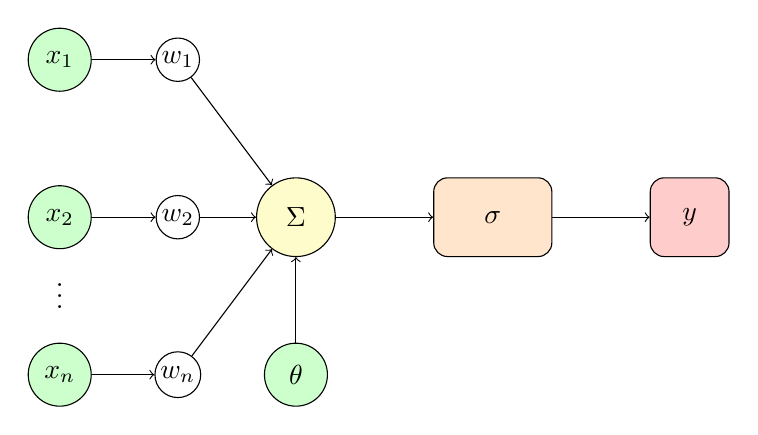
\begin{tikzpicture}[
    neuron/.style={circle, draw=black, fill=blue!20, minimum size=1.2cm},
    input/.style={circle, draw=black, fill=green!20, minimum size=0.8cm},
    weight/.style={fill=white, circle, draw=black, inner sep=1pt},
    arrow/.style={-Stealth, semithick},
    label/.style={text width=2cm, align=center, font=\small\sffamily}
]

\node[input] (x1) at (-3, 2) {$x_1$};
\node[input] (x2) at (-3, 0) {$x_2$};
\node at (-3, -0.9) {$\vdots$};
\node[input] (xn) at (-3, -2) {$x_n$};

\node[weight] (w1) at (-1.5, 2) {$w_1$};
\node[weight] (w2) at (-1.5, 0) {$w_2$};
\node[weight] (wn) at (-1.5, -2) {$w_n$};

\node[draw, circle, minimum size=1cm, fill=yellow!20] (sum) at (0, 0) {$\Sigma$};
\node[draw, rectangle, rounded corners=5pt, minimum width=1.5cm, minimum height=1cm, fill=orange!20] (act) at (2.5, 0) {$\sigma$};
\node[draw, rectangle, rounded corners=5pt, minimum width=1cm, minimum height=1cm, fill=red!20] (out) at (5, 0) {$y$};
\node[input] (b) at (0, -2) {$\theta$};

\draw (x1) edge[->] (w1);
\draw (x2) edge[->] (w2);
\draw (xn) edge[->] (wn);

\draw (w1) edge[->] (sum);
\draw (w2) edge[->] (sum);
\draw (wn) edge[->] (sum);

\draw (b) edge[->] (sum);
\draw (sum) edge[->] (act);
\draw (act) edge[->] (out);

\end{tikzpicture}
\caption{Representação gráfica de um neurónio de MacCough-Pitts. Fonte: elaborada pelos autores.}
\label{fig:neuronio-de-pitts}
\end{figure}

Formalizando matemáticamente a figura \ref{fig:neuronio-de-pitts},
sendo $W$ um vetor de pesos $\in [-1, 1]$, $\boldsymbol{x}$ um vetor de entradas
de tamanho $n$ e pertecente a $R^n$, $\theta$ um valor pertecente a $R$ 
e $\sigma$ uma função não linear. Um neurõnio é uma função $f: R^n \rightarrow R$,

\begin{eqnarray}\label{eq:neuronio-pitts}
    \sigma((\sum_{i=1}^{n} W_i\boldsymbol{x_i}) + \theta)
\end{eqnarray}

O termo $\theta$ pode ser entendido como o último elemento de $\boldsymbol{x}$ 
que está sendo sempre multiplicado pelo último elemento de $W$
que sempre tem valor igual a $1$, logo a equação \ref{eq:neuronio-pitts}
pode ser simplicada como,

\begin{eqnarray}\label{eq:neuronio-pitts-simplificado}
    \sigma(W\boldsymbol{x})
\end{eqnarray}

Um neurõnio pode ser entendido como uma transformação linear, a multiplicação
das entradas pelos pesos e viéses somados, seguida por uma
transformação não linear. Esta é feita pela função de ativação $\sigma$.
Alguns exemplos de funções de ativação empregradas nas redes neurais são A
função \textit{sigmoid} \ref{eq:sigmoid}, 
tangente hiperbólica (\textit{tanh}) \ref{eq:tanh}e 
\textit{Rectfied Linear Unit} (\textit{ReLU}) \ref{eq:relu}.

\begin{eqnarray}
    \text{sigmoid}(x) &=& \frac{e^x}{1 + e^x}\label{eq:sigmoid}
    \\
    \text{tanh}(x) &=& \frac{e^x - e^{-x}}{e^x + e^{-x}}\label{eq:tanh}
    \\ 
    \text{ReLU}(x) &=& \begin{cases} 
                        x & \text{if } x > 0 \\
                        0 & \text{if } x \leq 0 
                    \end{cases}\label{eq:relu}
\end{eqnarray}

Um único neurõnio não é capaz de aproximar qualquer função, para isso, eles são 
organizados em camadas que a saída de cada neurõnio de uma camada forma 
parte da entrada de todos os neurõnios da camada seguinte. 
A primeira camada apenas representa os dados de entrada, a última camada
representa um vetor de saída de tamanho 
Logo, uma rede neural \textit{feedfoward} com $L$ camadas escondidas 
pode ser entendida como uma função composta $f$ formada por 
um conjunto de consecutivas transformações lineares e não lineares num 
vetor de dados de entrada de tamanho $n$ $\boldsymbol{x} \in R^n$
que produz como saída um vetor de tamanho $m$ $\boldsymbol{\hat{y}} \in R^m$,  
sendo as transformações intermediárias representadas pelas saídas $y^l$ 
da camada escondida $l$, $l \in [1,..,L]$,

\begin{equation}\label{eq:rede-neural-composta}
    f(\boldsymbol{x}) = \sigma^{L + 1} y^{L + 1} \circ \sigma^{L} \circ y^{L} 
    \dots \circ \sigma^{2} \circ y^{2} \circ \sigma^{1} \circ y^{1}
\end{equation}

A figura \ref{fig:feedfoward-representacao-grafica} resume graficamente a
definição presente na equação \ref{eq:rede-neural-composta}.

\begin{figure}[htpb]
\centering
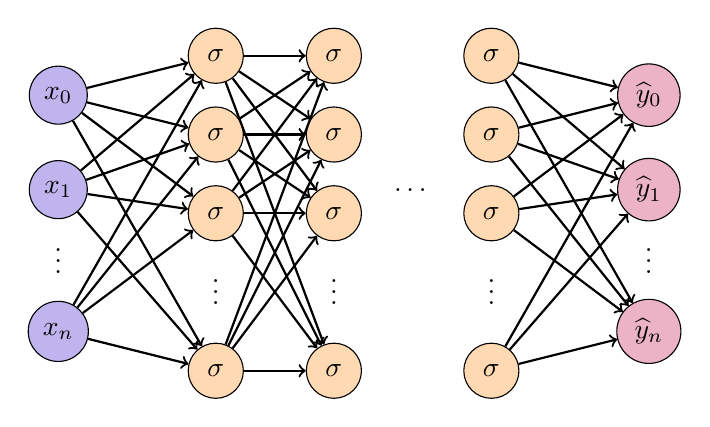
\begin{tikzpicture}[
    neuron/.style={circle, draw, minimum size=0.7cm},
    layer/.style={rectangle, minimum width=1.5cm, minimum height=8cm, draw=black, fill=blue!10, rounded corners=3pt},
    input/.style={neuron, fill=blue!30},
    hidden/.style={neuron, fill=orange!30},
    output/.style={neuron, fill=purple!30},
    physnode/.style={rectangle, draw, rounded corners, fill=orange!30, minimum width=1.5cm, minimum height=1.8cm},
    lossnode/.style={rectangle, draw, rounded corners, fill=yellow!30, minimum width=2cm, minimum height=3.2cm, align=center},
    every edge/.style={draw, ->, thick}
]

\node[input] (I-1) at (0, 3.5) {$x_0$};
\node[input] (I-2) at (0, 2.3) {$x_1$};
\node at (0, 1.5) {$\vdots$};
\node[input] (I-3) at (0, 0.5) {$x_n$};

\node[hidden] (H1-1) at (2, 4) {$\sigma$};
\node[hidden] (H1-2) at (2, 3) {$\sigma$};
\node[hidden] (H1-3) at (2, 2) {$\sigma$};
\node at (2, 1.1) {$\vdots$};
\node[hidden] (H1-4) at (2, 0) {$\sigma$};

\node[hidden] (H2-1) at (3.5, 4) {$\sigma$};
\node[hidden] (H2-2) at (3.5, 3) {$\sigma$};
\node[hidden] (H2-3) at (3.5, 2) {$\sigma$};
\node at (3.5, 1.1) {$\vdots$};
\node[hidden] (H2-4) at (3.5, 0) {$\sigma$};

\node at (4.5, 2.3) {$\dots$};

\node[hidden] (Hn-1) at (5.5, 4) {$\sigma$};
\node[hidden] (Hn-2) at (5.5, 3) {$\sigma$};
\node[hidden] (Hn-3) at (5.5, 2) {$\sigma$};
\node at (5.5, 1.1) {$\vdots$};
\node[hidden] (Hn-4) at (5.5, 0) {$\sigma$};

\node[output] (O-1) at (7.5, 3.5) {$\widehat{y}_0$};
\node[output] (O-2) at (7.5, 2.3) {$\widehat{y}_1$};
\node at (7.5, 1.5) {$\vdots$};
\node[output] (O-3) at (7.5, 0.5) {$\widehat{y}_n$};

% Connections
\foreach \i in {1,2,3}
    \foreach \j in {1,...,4}
        \path (I-\i) edge (H1-\j);

\foreach \i in {1,...,4}
    \foreach \j in {1,...,4}
        \path (H1-\i) edge (H2-\j);

\foreach \i in {1,...,4}
    \foreach \j in {1,...,3}
        \path (Hn-\i) edge (O-\j);

\end{tikzpicture}
\caption{Representação gráfica das redes \textit{feedfoward}. Fonte: elaborada pelos autores.}
\label{fig:feedfoward-representacao-grafica}
\end{figure}

O vetor de saída $\boldsymbol{\hat{y}}$ é então comparado com um vetor desejado 
$\boldsymbol{y}$ para calcular o erro entre a saída da rede e a saída desejada.
Este é o papel da função de perda (\textit{loss function}). 
Usualmente, para o caso de uma regressão, emprega-se a função de erro quadrático médio, 
do inglês, \textit{mean root square} (\textit{MSE}), como definida na equação
\ref{eq:mse}.

\begin{equation}\label{eq:mse}
    \mathcal{L} = MSE = \frac{1}{N} \sum_{i=0}^{N}(y_i - \hat{y}_i)^{2}
\end{equation}

Para problemas de classificação de classificação, aplica-se a função de entropia
cruzada (\textit{cross-entropy}) para problemas de classificação binária, sendo
$p$ e $q$ duas distribuições a função de perda é definida pela fórmula 
\ref{eq:cross-entropy}.

\begin{equation}\label{eq:cross-entropy}
    \mathcal{L} = \mathcal{H}(p,q) = - \sum_{x \in \mathcal{X}}{}p(x) \log q(x)
\end{equation}

Já para o caso de classificação com multiplos rótulos, aplica-se e a função 
de \textit{softmax}. Para um problema de classificação de multiplos rótulos com 
$N$ classes, a função de \textit{softmax} é definida pela fórmula \ref{eq:softmax}.

\begin{eqnarray}
    \rho_i &=& \frac{e^{z_i}}{\sum_{i=0}^{N}e^{z_j}} \\
    \mathcal{L} &=& arg max (\rho_0, \rho_1, \cdots, \rho_r) \label{eq:softmax}
\end{eqnarray}

A atualização dos pesos de cada camada se dá pela cálculo do grandiente
de uma função de erro $\mathcal{L}$. O "tamanho do passo" que será dado
é determinado por um parâmetro $\alpha$ chamado de taxa de aprendizagem.
O conjunto de pesos $W$ é então atualizado segundo a fórmula 
\ref{eq:atualizacao-parametros-redes},

\begin{equation}\label{eq:atualizacao-parametros-redes}
    W_{t + 1} = W_{t} + \alpha \nabla \mathcal{L}
\end{equation}

A propagação dos erros se dá pelo algoritmo de retropropagação, sendo um caso 
de aplicação da regra da cadeia. A derivada da função de perda $\mathcal{L}$ de 
uma rede com $L$ camadas escondidas pode ser expressa então pela fórmula 
\ref{eq:derivida-loss}.

\begin{equation}\label{eq:derivida-loss}
    \frac{d\mathcal{L}}{d\sigma^{L}} \cdot 
    \frac{d\sigma^{L}}{dy^{L}} \cdot
    \frac{dy^{L}}{d\sigma^{L-1}} \cdot
    \frac{d\sigma^{L-1}}{dy^{L-1}} \cdot
    \frac{dy^{L-2}}{dy^{L-2}} \cdot
    \cdots
    \frac{d\sigma^{1}}{dy^{1}} \cdot
    \frac{dy^{1}}{dx}
\end{equation}

A atualização dos pesos se dar por meio da avaliação da expressão acima da esquerda 
para a direita, computando o gradiente $\delta$ em cada camada $l$ e pesos $W^l$
como descrito pela equação
\ref{eq:gradiente-camada}

\begin{equation}\label{eq:gradiente-camada}
    \delta_{l} = (\sigma^l)' \circ (W^{l+1}) \dot (\sigma^{l + 1})' \circ 
    \cdots 
    \circ (W^{L-1}) \dot (\sigma^{L-1})' 
    \circ (W^{L}) \dot (\sigma^{L})'
    \circ \nabla \mathcal{L}
\end{equation}

A atualização dos pesos $W$ da camada $l$ utilizando os gradientes $\delta_l$ 
pode ser expresso pela equação \ref{eq:atualizacao-camada}.

\begin{equation}\label{eq:atualizacao-camada}
    \nabla_W \mathcal{L} = \delta_l (\sigma^{l-1}) 
\end{equation}

\section{Redes Neurais Informadas pela Física}

Apresentadas em \cite{raissi-etal:19}, PINNs podem ser entendidas como uma forma
avançada de regularização, ou como um problema de otimização que transforma 
as condições de fronteira e iniciais em penalizações para a função custo. 

\subsection{PINNs como Solucionadores de Equações Diferenciais}

Cabe aqui prover uma definição formal do que são equações diferencias e como as 
PINNs resolvem este tipo de equação. 
PINNs são capazes de resolver problemas no seguinte formato: 

\begin{eqnarray}
    \mathcal{D}(u(\boldsymbol{x},t);\boldsymbol{\lambda}) &=& f(u,\boldsymbol{x},t), \quad \boldsymbol{x} \in \Omega, \, t \in I, \label{model-1-a}\\
    %
    \mathcal{B}(u(\boldsymbol{x},t)) &=& g(\boldsymbol{x},t), \quad \boldsymbol{x} \in \Gamma, \, t \in I, \label{model-1-b}\\
    %
    \mathcal{I}(u(\boldsymbol{x},t_0)) &=& q(\boldsymbol{x}), \quad \boldsymbol{x} \in \Omega, \label{model-1-c}
\end{eqnarray}

Em que $\Omega \subset \mathbb{R}^d$ é o domínio espacial limitado pela 
fronteira $\Gamma$; 
$d$ é a dimensão do domínio espacial; 
$T = [t_0, t_f]$ é o intervalo de tempo, sendo $t_0 < t_f$; 
$\boldsymbol{x} = (x_1, x_2, \dots, x_d)$ é um vetor de coordenadas espaciais; 
$t$ denota o tempo; 
$u = u(\boldsymbol{x}, t)$ denota a solução desconhecida do problema; 
$\boldsymbol{\lambda}$ é um vetor de parâmetros das equações; 
$\mathcal{D}$ é um operador diferencias associado às equações; 
$f$ é um termo fonte ou sorvedouro; 
$\mathcal{B}$ and $\mathcal{I}$ são operadores representando, respectivamente,
as condições de fronteira e iniciais; 
por fim, $g$ e $q$ são funções conhecidas que definem essas condições.

A equação \ref{eq:loss-fisica} define o termo da função de perda que engobla
todos as equações que compõem o modelo. Trata-se de um treinamento 
não-supervisionado que busca minimizar o residual definido.

\begin{equation}\label{eq:loss-fisica}
    \mathcal{L}_{\text{física}}(\boldsymbol{\theta}) 
    = \mathcal{L}_{\mathcal{D}}(\boldsymbol{x},t,\boldsymbol{\theta}) 
    + \mathcal{L}_{\mathcal{B}}(\boldsymbol{x},t,\boldsymbol{\theta}) 
    + \mathcal{L}_{\mathcal{I}}(\boldsymbol{x},t_0,\boldsymbol{\theta}) 
    %+ \omega_{data} J_{data}(\boldsymbol{x},t,\boldsymbol{\theta})
\end{equation}

Sendo $\omega_{\text{domínio}}$, $\omega_{\text{fronteira}}$ 
e $\omega_{\text{inicial}}$ pesos atribuídos a cada um dos residuais.
Caso haja dados disponíveis, é feito um treinamento supervisionado utilizando 
tais dados. A função de perda final da rede neural é então definida pela equação
\ref{eq:loss-total}.

\begin{eqnarray}\label{eq:loss-total} 
    \mathcal{L}_{\text{total}}(\boldsymbol{\theta}) 
    = \omega_{\text{física}} \mathcal{L}_{\text{física}}(\boldsymbol{\theta}) 
    + \omega_{\text{dados}} \,\mathcal{L}_{\text{dados}}(\boldsymbol{\theta})
\end{eqnarray}

Aqui vale menciona que esta não é a única forma de distribuir os pesos da loss,
a implementação da biblioteca \textit{DeepXDE} \cite{lu-etal:21-deepxde}
permite atribuir pesos diferentes a cada condição inicial e de fronteira. 
Então o problema passa a ser encontrar os conjuntos $\boldsymbol{\theta}^*$ de 
parâmetros e viéses da rede que minimiza a função \ref{eq:loss-total}.

\begin{equation}\label{eq:otimizacao-parametros}
   \boldsymbol{\theta}^* 
   = \arg \min_{\boldsymbol{\theta}} \mathcal{L}_{\text{total}}(\boldsymbol{\theta}), 
\end{equation}

Existem muitos métodos de otimização para encontrar os argumentos 
da equação \ref{eq:otimizacao-parametros}. Pode-se citar o método de 
primeira ordem \textit{Adam} \cite{kingma-ba:14-adam} e o método quase-newtoniano
\textit{BFGS}, ou como comumente usado, a sua versão para ambientes de pouca
memória, o \textit{L-BFGS} \cite{liu-nocedal:89-lbfgs}.

A figura \ref{fig:pinn-representacao-grafica} mostra uma representação gráfica das 
PINNs.

\begin{figure}[htpb]
\centering
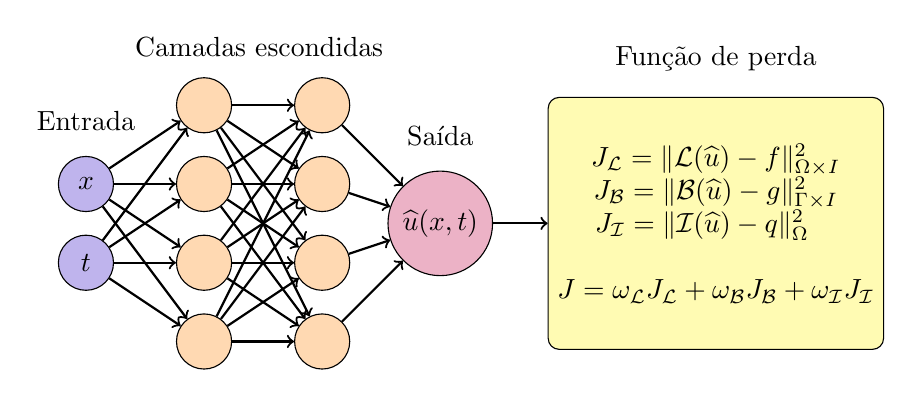
\begin{tikzpicture}[
    neuron/.style={circle, draw, minimum size=0.7cm},
    input/.style={neuron, fill=blue!30},
    hidden/.style={neuron, fill=orange!30},
    output/.style={neuron, fill=purple!30},
    physnode/.style={rectangle, draw, rounded corners, fill=orange!30, minimum width=1.5cm, minimum height=1.8cm},
    lossnode/.style={rectangle, draw, rounded corners, fill=yellow!30, minimum width=2cm, minimum height=3.2cm, align=center},
    every edge/.style={draw, ->, thick}
]

\node[input] (I-1) at (0, 2) {$x$};
\node[input] (I-2) at (0, 1) {$t$};

\node[hidden] (H1-1) at (1.5, 3) {};
\node[hidden] (H1-2) at (1.5, 2) {};
\node[hidden] (H1-3) at (1.5, 1) {};
\node[hidden] (H1-4) at (1.5, 0) {};

\node[hidden] (H2-1) at (3, 3) {};
\node[hidden] (H2-2) at (3, 2) {};
\node[hidden] (H2-3) at (3, 1) {};
\node[hidden] (H2-4) at (3, 0) {};

\node[output] (O-1) at (4.5, 1.5) {$\widehat{u}(x,t)$};

% Connections
\foreach \i in {1,2}
    \foreach \j in {1,...,4}
        \path (I-\i) edge (H1-\j);

\foreach \i in {1,...,4}
    \foreach \j in {1,...,4}
        \path (H1-\i) edge (H2-\j);

\foreach \j in {1,...,4}
    \path (H2-\j) edge (O-1);

\node[lossnode] (TotalLoss) at (8, 1.5) {
$J_{\mathcal{L}} = \lVert \mathcal{L}(\widehat{u}) - f \rVert^{2}_{\Omega \times I}$
\\
$J_{\mathcal{B}} = \lVert \mathcal{B}(\widehat{u}) - g \rVert^{2}_{\Gamma \times I}$
\\
$J_{\mathcal{I}} = \lVert \mathcal{I}(\widehat{u}) - q \rVert^{2}_{\Omega} \quad$
\\
\\
$J = \omega_{\mathcal{L}} J_{\mathcal{L}} + \omega_{\mathcal{B}} J_{\mathcal{B}} + \omega_{\mathcal{I}} J_{\mathcal{I}}$
};

\path (O-1) edge (TotalLoss);

% Labels
\node[above=0.2cm] at (I-1.north) {Entrada};
\node[above=0.2cm] at (2.2, 3.3) {Camadas escondidas};
\node[above=0.2cm] at (O-1.north) {Saída};
\node[above=0.2cm] at (TotalLoss.north) {Função de perda};

\end{tikzpicture}
\caption{Representação gráfica das PINNs. Fonte: elaborada pelos autores.}
\label{fig:pinn-representacao-grafica}
\end{figure}

\subsection{Formulação para Problemas Inversos}

A formulação para as PINNs apresentada até então foca na resolução de problemas
diretos. Em \cite{raissi-etal:19} é apresentada uma extensão para a mesma que 
também soluciona problemas inversos. Solucionar um problema inverso consiste em,
dado um conjunto de dados representados pela $\mathcal{L}_{\text{dados}}$,
encontrar um conjunto de parâmetros $\boldsymbol{\lambda}$ que minimaniza a
$\mathcal{L}_{\text{total}}$.
A equação \ref{eq:loss-total} pode então ser reescrita como,

\begin{eqnarray}\label{eq:loss-total-problema-inverso} 
    \mathcal{L}_{\text{total}}(\boldsymbol{\theta}, \boldsymbol{\lambda}) 
    = \omega_{\text{física}} \mathcal{L}_{\text{física}}(\boldsymbol{\theta}, \boldsymbol{\lambda}) 
    + \omega_{\text{dados}} \,\mathcal{L}_{\text{dados}}(\boldsymbol{\theta})
\end{eqnarray}

O problema de minimização descrito em \ref{eq:otimizacao-parametros} passa 
então a ser encontrar o conjunto $\boldsymbol{\theta}^*$ de parâmetros da rede,
como também o conjunto $\boldsymbol{\lambda}^*$
que minimiza a função \ref{eq:loss-total-problema-inverso}, 

\begin{equation}\label{eq:otimizacao-parametros-problema-inverso}
   (\boldsymbol{\theta}^*, \boldsymbol{\lambda}^*) 
   = \arg \min_{\boldsymbol{\theta}, \boldsymbol{\lambda}} \mathcal{L}_{\text{total}}(\boldsymbol{\theta}, \boldsymbol{\lambda}), 
\end{equation}

Vale salientar que a rede ao encontrar os conjuntos $\boldsymbol{\theta}^*$
e $\boldsymbol{\lambda}^*$, a rede neral está solucionando tanto o problema
direto (aproximar uma função que satisfaça as equações diferencias), quanto o 
problema inverso (encontrar $\boldsymbol{\lambda}^*$). 

\subsection{Pontos de Colocação}

Pontos de colocação são um conceito importante para as PINNs, sendo análogos
a criação da malha do \textit{MEF}. Entretanto, diferente do \textit{MEF}, 
não há um critério método bem definido para a obtenção destes pontos. 
Os pontos de colocação podem ser entendidos como uma discretização do domínio
de uma equação diferencial. O único critério que deve ser atendido é o uso
de pontos nas condições de fronteira e iniciais do problema.
Por esta perspectiva, os pontos de colocação podem ser entendidos como uma 
amostra do domínio na qual a rede neural será treinada. 
Por este motivo, muitas técnicas de amostragem multidimensional são 
aplicadas às PINNs para definir os pontos de colocação, pode-se citar como 
exemplo o hipercubo latino.

\section{Arquiteturas Alternativas}

A definição de PINNs como uma rede neural com informação física não se aplica
apenas a redes \textit{feedfoward}, qualquer arquitetura de redes neurais
que incorpora as equações que descrevem os dados em que rede está sendo treinada, 
pode ser considerada uma rede neural informada pela física, uma PINN.
Desde a publicação do artigo seminal em 2019, uma série de arquiteturas 
alternativas foram propostas utilizando a ideia das PINNs como princípio.

Uma classe de EDPs de especial interesse para áreas como teoria dos campos quânticos
e mecânica estatística são as EDPs estocásticas. Esta classe de equações diferenciais
pode ser entendida como uma equação diferencial com um termo $\xi$ que representa
um campo com ruído. 
O exemplo mais simples é a equação do calor estocástica \ref{eq:difusao-estocastica}.
\begin{equation}\label{eq:difusao-estocastica}
    \frac{\partial u}{\partial t} = \nabla \cdot u + \xi
\end{equation}
Uma proposta de PINNs para EDPs estocásticas é apresentada em \cite{zhang-etal:2020-stochastic-pde-pinns},
em que são empregados métodos espectrais ortogonais para modelar processos que 
representam a estocasticidade nos dados. Estes processos são incorporados à função 
de perda como termos regularizadores extras.  
Outra arquitetura pensada para a solução de EDPs estocásticas são as FINNs,
apresentadas em \cite{karlbauer-2022-finns}, que combinam o método de volumes finitos
com redes neurais para obter soluções para problemas de advecção-difusão como a
equação de \textit{Burgers} e de \textit{Allen-Cahn}.
A arquitetura obteve resultados superiores a redes neurais sem informação física
e até mesmo de PINNs convencionais.   

Um exemplo de proposta de PINNs alternativas que explora limitações das PINNs 
originais pode ser encontrada em \cite{sun-e-feng:2023-gPINNs}.
Os autores propõem as gPINNs (Gradient Enhanced PINNs) que tentam contornar as 
complexidades dos algoritmos de diferenciação automática existentes para equações de alta 
ordem. A arquitetura utiliza uma função de ativação adaptativa, uma técnica de 
melhoria nos gradientes para acelerar a convergência do modelo, e uma técnica 
chamada de \textit{deep mixed residual method} para compensar o \textit{overhead}
gerado pela melhoria nos gradientes. A arquitetura é empregada na solução de 
equações de onda da luz.
Outra proposta similar que também explora o uso de melhorias no gradientes pode 
ser encontrada em \cite{mohammadian-etal:2023-gradient-enhanced}, tendo como
maior vantagem a necessidade de poucos dados para treinamento, acelerando o processo
de treinamento.
Os autores utilizam o método proposto para gerar estimativas para sistemas de 
controle de redes elétricas.  

Técnicas como convolução e recorrência, comuns em áreas como visão computacional 
e processamento de linguagem natural, também encontram espaço na solução de problemas
científicos. Em \cite{ren-etal:2022-phycrnet} são propostas as PhyCRNet e PhyCRNet-s
para resolução de EDPs sem dados de treinamento. A arquitetura emprega uma rede
LSTM \textit{enconder-decoder} com convolução para a extração de características
espaciais e simulação da evolução do fenômeno no tempo.
Para evitar o ajuste de hiper-parâmetros, as condições iniciais e de contorno não
são impostas por meio de penaliadades na função custo, mas como \textit{hard-constraints}.
Também são utilizadas conexões residuais e autoregressivas para simular a progressão
do tempo. OS autores obtiveram resultados satisfatórios para problemas como a 
equação de \textit{Burgers} e problemas de reação-difusão.
Outro exemplo envolvendo camadas convolucionais pode ser encontrado em 
\cite{shi-etal:24-convnet}. No artigo é proposto uma arquitetura em que uma única 
camada convolucional é empregada. Nos testes realizados pelos autores, a rede 
neural proposta apresentou uma convergência melhor do que uma PINN convecional 
para problemas de difusão com diferentes frequências.

Pensanda para lidar com problemas ligadas a solução de PDEs com dados que possuem 
componentes com fequências diferentes, a arquitetura proposta em \cite{han-etal:2023-hierarchical-learning}
utiliza aprendizado hierarquico para lidar com esse problema.
O princípio por de trás do aprendizado hierarquico é utilizar camadas com redes
neurais responsáveis por aproximar uma frequência, assim cada camada 
adicionada deve aprender a partir dos dados residuais da camada anterior.
A saída dessas camadas é então alimentada em uma rede de características de Fourier
embutidas. 
As primeiras camadas capturam os componentes de menor frequência, enquanto que
que a rede de características embutidas fica responsável por impor limites a solução.
A arquitetura proposta é testada com uma série de equações diferenciais parciais.

Outro exemplo de arquiteturas alternativas de redes neurais com informação física
pode ser encontrada em \cite{benjamin-etal:2022-rnn-dct-networks}. 
Os autores propoêm as \textit{rnn-dct networks}, que combinam a arquitetura clássica
de redes residuais (RNN) e DCT (\textit{discrete cossine transformations}) com 
redes MLP (feedfoward). O DCT é responsável por codificar a parte espacial da equação,
enquanto que a RNN fica responsável por interpretar os valores temporais.
O resultado dessas duas redes são então combinados e usados para alimentar a rede
\textit{feedfoward}, ajudando esta a capturar as relações espaciais e temporais do
problema. A arquitetura proposta apresentou resultados execelentes em problemas 
envolvendo as equações de Navier-Stokes, como o problema de vortices de Taylor-Green.

Em \cite{pakravan-et:2021-bipde} é apresentado um método focado na solução de 
problemos inversos envolvendo EDPs com lacunas nos dados chamado 
\textit{Blended inverse-PDE networks} BiPDE.
Os parâmetros da equação são descobertos utilizando não apenas conhecimentos sobre
a física incorporados a função de perda, mas também utilizando conhecimentos específicos 
do domínio. 
A rede neural exerce o papel de aproximador universal dos parâmetros, que combinado 
com um solucionador de EDPs, livra a rede de ter que resolver o problema de 
forma direta, focando apenas no problema inverso, tornando o método mais eficiente,
ao não necessitar de tantos dados para o treinamento.
O método proposto é testado em problemas inversos envolvendo encontrar coeficientes
de difusão variantes para as equações de \textit{Burgers} e de \textit{Poisson}, 
além de problemas de alta dimensionalidade.

Propostas em \cite{jagtap-etal:2020-convervative-pinns}, as conservative PINNs 
(cPINNs) utilizam leis de conservação não-lineares para a solução de problemas 
em domínios discretos. Para aplicar as cPINNs, o domínio é fragmentado em subdomínios
nos quais as cPINNs aão empregadas, a propriedade de conversão é garantida pela 
aplicação de continuidade ao longo de todos os subdomínios. Nas fronteiras entre
os subdomínios, a solução é obtida pela média das saídas de cada cPINN.
Uma vantagem desta arquitetura é permitir que em cada subdomínio sejam utilizados
diferentes meta-parãmetros, como número de camadas escondidas, funcões de ativação
e otimizadores.
A arquitetura é capaz de tirar grade proveito de processamento paralelo.  

Utilizando as cPINNs como base, as \textit{Extended Physics-informed Neural Networks}
(XPINNs) são propostas em \cite{jagtap-etal:2020-extended-pinns}. Assim como as 
cPINNs, o domínio é fragmentado em subdomínios permetindo que a otimização dos
meta-parâmetros possa ser feita em cada rede. 
A grande novidade da arquitetura é a possibilidade de aproximar qualquer EDP.
Outra novidade é a decomposição arbritária do domínio, o que permite tirar ainda
mais profeito de paralelismo durante o treinamento do modelo.
A arquitetura foi aplicada em PDE não-lineares com geometrias complexas, 
aproveitando a decomposição de domínio.
Continuando o desenvolvimento da arquitetura, em \cite{hu-etal:2023-augmented-pinns}
são propostas as \textit{Augmented PINNs} (APINNs), a novidade da arquitetura 
é tornar a fragmentação dos subdomínios treinável.
A arquitetura permite que dados de treinamento sejam usados entre diferentes 
fragmentos, aumentando a generalização do modelo.
A performance das APINNs é consideravelmente superior a das XPINNs em termos 
de fragmentação do domínio e generalização.

Aproveitando as possibilidades que o uso de paralelismo pode trazer em termos 
de velocindade no tempo de treinamento, em \cite{dwivedi:2019-distributed-pinns}
são propostas as Distribuited PINNs (DPINNs). A principal ideia por trás deste método
é fragmentar o domínio do problema em partes que devem ser aproximadas por uma rede
neural independente. Uma vantagem dessa abordagem é que é possível utilizar redes
mais simples em cada fragmento, ao invés de aplicar uma única rede mais complexa
para todo o domínio. A função de perda é calculada com base na aproximação de cada
rede neural que funcionam como PINNs paralelas. O método é capaz de aproximar 
corretamente problemas difícies como as equações de Navier-Stokes de forma satisfatória
utilizando redes simples, obtendo resultados melhores do que aqueles com uma
rede neural informada pela física centralizada.

Problemas de engenharia costumam ter parâmetros incertos que são dependentes 
de variáveis temporais e espaciais, estas incertezas são contornadas utilizando
processos que as modelam.
Métodos como o MEF são capazes de resolver tais equações, mas é necessário ter um
conhecimento \textit{a priori} sobre as distribuições que modelam o fenômeno estudado,
fazendo com que métodos puramente estátiscos sejam insuficientes.
É comum empregar técnicas como teoria de conjuntos difusos junto aos métodos 
tradicionais de solução de equações diferenciais.
Aproveitando o potencial que as PINNs e conjuntos difusos tem para a soluções 
de equações com tais características, em \cite{fugh-etal:2022-fuzzy-pinns} 
são propostos dois novos modelos as 
\textit{Interval Physics-Informed Neural Networks} (iPINNs) e 
\textit{Fuzzy Physics-Informed Neural Networks} (fPINNs) que combinadas, 
são capazes de resolver problemas envolvendo equações diferencias e conjuntos 
difusos sem conhecimentos prévios. Uma rede neural é responsável pela a aproximação 
das entradas, enquanto a outra fica responsável por aproximar a solução da PDE.  
O método proposto mantêm as vantagens das PINNs, como não precisar de uma 
malha de pontos, e ser capaz de resolver problemas de forma direta e inversa
sem alterações significativas nos métodos.

As equações de ordem fracionaria, também chamadas de equações diferenciais 
extraordinárias, são uma classe de equações diferencias que encontram aplicações 
na modelagem de diversos fenõmenos físicos como escoamentos subterrâneos 
\cite{atangana-2013-fluxo-ordem-fracionaria} e equações de conservação de massa
\cite{wheatcraft-2008-conservacao-de-massa-fracionaria}. 
A equação \ref{eq:exemplo-ordem-fracionaria} mostra a forma geral para tais equações.
\begin{equation}\label{eq:exemplo-ordem-fracionaria}
    \dfrac{d^{\alpha}u}{dx^{\alpha}} = u, \quad \alpha \in \mathbb{R}
\end{equation}
Em \cite{pang-etal:2019-fPINNs} é proposto uma arquitetura de redes neurais 
informadas pela física pensada para equações diferenciais de ordem fracionária.
O principal entrave para o uso de PINNs convecionais na solução dessas equações
está ligado ao fato de que algoritmos de diferenciação automática são otimizados
para equações de ordem inteira.
A arquitetura proposta, chamado de \textit{fPINNs}, contorna tais limitações ao
aplicar uma abordagem mista que utiliza diferenciação automática para a parte inteira
das derivadas e derivadas númericas para a parte fracionária.
A arquitetura proposta foi capaz de solucionar problemas clássicos como a equação de 
\textit{Burgers} utilizando derivadas parciais de ordem fracionária, obtendo
resultados equiparáveis ao MEF.

Baseado nas \textit{KANs} (\textit{Kolmogorov-Arnold Neural Networks})
\cite{liu-etal:2025-kans}, redes neurais baseadas no teorema de representação 
universal de Kolmogorov-Arnold, foram propostas as \textit{PIKANs} 
(\textit{Physically Informed Kolmogorov-Arnold Neural Networks})
que combinando as funcões de ativação baseadas em \textit{b-splines} das
\textit{KANs} com a técnica de regressão simbólica, permite encontrar  
representações analíticas das soluções encontradas pela rede neural.
As KANs não se mostraram superiores aos MLPs para todo tipo de tarefa 
\cite{toscano:2025-pinns-para-pikans}, mas sua superiodade com regressão simbólica
demonstra o potencial da arquitetura para problemas envolvendo explicabilidade.



\chapter{Modelos Compartimentais}
\label{sec-modelos-compartimentais}

Neste cápitulo são apresentados os principais conceitos acerca dos modelos compartimentais
para a compreensão do trabalho desenvolvido nesta dissertação. No fim do cápitulo
é apresentada uma pequena revisão de aplicação de PINNs com modelos compartimentais.

\section{Origens}

Apresnetado no conjunto de trabalhos seminais \cite{kermack-mcKendrick:1927}, 
\cite{kermack-mcKendrick-pt2:1932} e \cite{kermack-mcKendrick-pt3:1933} e consolidados
em estudos como \cite{kendall:2023-modelos-epd-estocasticos}, 
modelos Compartimentais nada mais são do que modelos epidemiológicos utilizados 
no estudo de doenças contagiosas que separam a população em grupos.
Os fluxos de indivíduos entre esses grupos, chamados de compartimentos, são modelados 
por meio de operações de diferenciação.

\section{O modelo SIR}

Apresentado no trabalho seminal de \cite{kermack-mcKendrick:1927}, 
o modelo \textit{SIR} (Susceptible-Infected-Recovered) é definido pelo conjunto 
de equações \ref{eq:SIR-1}, \ref{eq:SIR-2} e \ref{eq:SIR-3}.

\begin{eqnarray}\label{eq:sir}
   \frac{dS(t)}{dt} &=& \frac{-\beta S(t)}{N} I(t),  \quad t > t_0, \label{eq:SIR-1}\\
   \frac{dI(t)}{dt} &=& \frac{\beta S(t)}{N} I(t) - \gamma I(t), \quad t > t_0, \label{eq:SIR-2}\\
   \frac{dR(t)}{dt} &=& \gamma I(t),  \quad t > t_0, \label{eq:SIR-3}
\end{eqnarray}

Estas três equações formam um sistema de equações diferencias de fácil interpretação.
A primeira equação modela a iteração entre pessoas infectadas e pessoas suscetíveis,
o parâmetro $\beta$, a taxa de infecção, diz quantos destes encontros resultaram 
em novos casos da doença. 
A terceira equação modela a recuperação de individuos ao
longo do tempo, o parâmetro $\gamma$ é taxa de individuos que se recuperam por 
unidade de tempo, sendo que a recuperação pode ser a cura da doença ou o falecimento
do individuo, já que o \textit{SIR} não distinguir os dois casos. 
A segunda equação é a soma do primeira e da terceira equação, mas com seus sinais
trocados. Ela modela o fluxo de indivíduos que entram e saem do compartimento
de infectados.  

Por se tratar de um sistema de equações diferencias ordinárias com três equações,
são necessárias três condições iniciais para se obter um problema de valor
inicial.

\begin{eqnarray}
   S(0) &=& S_0 \label{eq:SIR-S0}\\
   I(0) &=& I_0 \label{eq:SIR-I0}\\
   R(0) &=& R_0 \label{eq:SIR-R0}
\end{eqnarray}

Como o modelo não inclui mortes naturais ou por outras causas que não a doença
que está sendo modelada, nem o nascimento de pessoas na população estuda, assume-se
que a soma dos três comparimentos para qualquer tempo $t$ é igual ao total 
$N$ da popuiação,

\begin{equation}
   S(t) + I(t) + R(t) = N,  \quad t > t_0, \label{eq:SIR-4}
\end{equation}

O modelo pode ser entendido com um grafo em que os individuas fluem de um 
compartimento para outro a uma taxa $\beta$ e $\gamma$. 
A figura \ref{fig:sir-grafo} representa o \textit{SIR} por esta perspectiva.

\begin{figure}[H]
\centering
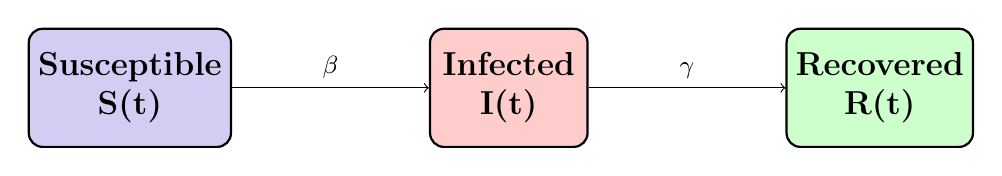
\begin{tikzpicture}[
    node distance=2.5cm,
    box/.style={rectangle, minimum width=2cm, minimum height=1.5cm, 
                draw=black, thick, align=center, rounded corners=5pt,
                font=\large\bfseries},
    arrow/.style={-Stealth, thick, line width=1.2pt},
    label/.style={midway, sloped, font=\small}
]

    % Define nodes
    \node[box, fill=blue!20] (S) {Susceptible \\ S(t)};
    \node[box, fill=red!20, right=of S] (I) {Infected \\ I(t)};
    \node[box, fill=green!20, right=of I] (R) {Recovered \\ R(t)};

    % Transitions
    \draw (S) edge[->] node[label,above] {$\beta$} (I);
    \draw (I) edge[->] node[label,above] {$\gamma$} (R);

\end{tikzpicture}
\caption{Grafo para o \textit{SIR}. Fonte: elaborada pelos autores.}
\label{fig:sir-grafo}
\end{figure}

Certas definições são necessárias neste ponto para se compreender os modelos compartimentais. 
Em modelos epidemiológicos, incidência é o fluxo de novos casos por unidade de tempo,
enquanto que a prevalência é a quantidade de casos na população num instante $t$.
No caso do \textit{SIR}, estes conceitos são representados respectivamente pelo
termo $\frac{-\beta S(t)}{N}$ e pela equação $I(t)$. 

O número de reprodução básico $R_0$ é defido como a relação entre os parametros
$\beta$ e $\gamma$. Ele é de particular interesse para o estudo da propagação
de uma doença, pois se $R_0 > 1$, significa que a dispersão da doença
ainda está em curso e o número de infectados tende a aumentar. 
Se $R_0 < 1$, significa que a dispersão já atigiu seu pico e o número de individuos
infectados tender a diminuir. Se $R_0 = 1$ a doença está em equilíbrio e o número 
de infectados tender a se manter o mesmo.

\begin{equation}\label{eq:numero-reproducao-basico}
    R_0 = \frac{\beta}{\gamma}
\end{equation}

Um valor relacionado ao número de reprodução básico $R_0$, é o número de reprodução
efetivo $R_e$. Enquanto que o número de reprodução básico $R_0$ é utilizado para
medir o dispersão de uma doença no início de uma pandemia. 
Seu valor é obtido pela multiplicação de $R_0$ por $S$ num instante $t$.

\begin{equation}\label{eq:numero-reproducao-efetivo}
    R_e = R_0 S(t)
\end{equation}

O limite $\mathcal{T}$ define o valor máximo de indivíduos que estarão contaminados
no pico da pandemia. Este limite é importante para tomadores de decisão e governos
para entender os efeitos sobre os serviços de saúde pública.

\begin{equation}
    \mathcal{T} = \frac{\gamma}{\beta}N = \frac{N}{R_0}
\end{equation}

A figura \ref{fig:exemplo-sir} mostra um exemplo do \textit{SIR} com $\beta=0.8$
e $\gamma=0.1$ e as três curvas características desse modelo.

\begin{figure}[H]
\centering
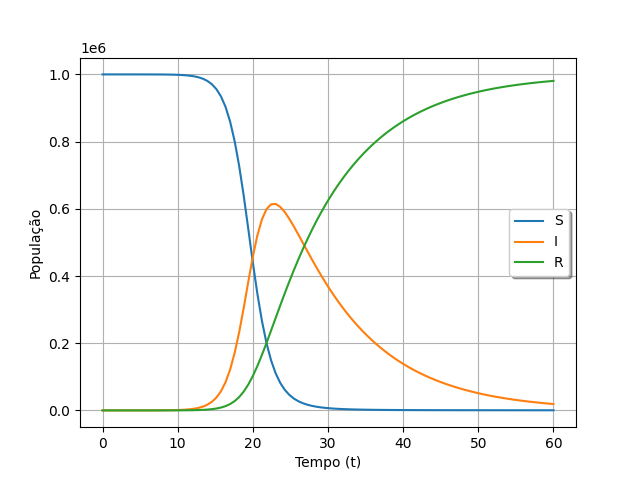
\includegraphics[width=0.6\textwidth]{figuras/sir-example-beta0.8-gamma0.1.png}
\caption{Exemplo do SIR com $\beta=0.8$ e $\gamma=0.1$.}
\label{fig:exemplo-sir}
\end{figure}

\section{Pontos de equilíbrio}

Os modelos compartimentais possuem dois pontos de equilíbrio chamados de 
ponto de equilíbrio livre de doenças (\textit{Deacese Free Equilibrium}) e 
ponto de equilíbrio endemico (\textit{Endemic Equilibrium}). 
O primeiro ponto é atingido quando não há mais indivíduos infectados na população,
ou seja, nos ponto em que $I$ é igual a zero. O ponto de equilíbrio endêmico
é atigindo justamente quando o número de novos casos é compensado pelo número
de indivíduos que se recuperam, mantendo o número de indivíduos no compartimento
\textit{Infected} constante, mas diferente de zero.

\section{Pontos críticos}

Utilizando o foi desenvolvido na seção anterior, pode-se facilmente encontrar os 
pontos críticos do modelo SIR. Considerando que os pontos de equilíbrio do modelo 
SIR são determinados pela solução do sistema composto pelas equações
\ref{eq:SIR-pontos-criticos-1}, \ref{eq:SIR-pontos-criticos-2} e \ref{eq:SIR-pontos-criticos-3}.

\begin{eqnarray}
    -\beta SI &=& 0 \label{eq:SIR-pontos-criticos-1}\\
    \beta SI - \gamma I &=& 0 \label{eq:SIR-pontos-criticos-2}\\
    \gamma I &=& 0 \label{eq:SIR-pontos-criticos-3}
\end{eqnarray}

A última equação $\gamma I=0$ implica que $I=0$. Substituindo este valor na primeira e 
segunda equações, as equações são satisfeitas para qualquer valor de S. 
Portanto, o sistema tem um conjunto de pontos de equilíbrio da forma:

\begin{equation}\label{eq:sir-conjunto-solucoes-eq-livre-doenca}
    (S* , I*, R*) = (S* , 0, R*)    
\end{equation}

Sendo $S* + R* = N$, ou seja, qualquer ponto em que não haja infectados e a soma 
dos suscetíveis e recuperados seja igual a N representa um estado de equilíbrio. 
Isso significa que o sistema pode estabilizar-se em diferentes estados dependendo 
da quantidade de indivíduos que permaneceram suscetíveis ou que foram recuperados. 
Esse é o estado de equilíbrio livre de doença, onde toda 
população está no compartimento \textit{Susceptible} ou \textit{Recovered} e não 
há mais infectados.

A análise de estabilidade dos pontos de equilíbrio do modelo SIR pode ser facilmente 
feita através da matriz jacobiana do sistema de equações diferencias. 
Considere a matriz \ref{eq:jacobiana-sir}.

\begin{equation}\label{eq:jacobiana-sir}
J(S,I,R) = 
\begin{bmatrix}
\frac{\partial f_1}{\partial S} & \frac{\partial f_1}{\partial I} & \frac{\partial f_1}{\partial R} \\[0.5em]
\frac{\partial f_2}{\partial S} & \frac{\partial f_2}{\partial I} & \frac{\partial f_2}{\partial R} \\[0.5em]
\frac{\partial f_3}{\partial S} & \frac{\partial f_3}{\partial I} & \frac{\partial f_3}{\partial R}
\end{bmatrix}
=
\begin{bmatrix}
-\beta I & -\beta S & 0 \\
\beta I & \beta S - \gamma & 0 \\
0 & \gamma & 0
\end{bmatrix}
\end{equation}

Utilizando a equação \ref{eq:sir-conjunto-solucoes-eq-livre-doenca} e aplicando-a
na matriz \ref{eq:jacobiana-sir}, chega-se ao ponto de equilíbrio 
\ref{eq:equilíbrio-sir}.

\begin{equation}\label{eq:equilíbrio-sir}
J(S*,0,R*)
=
\begin{bmatrix}
0 & -\beta S & 0 \\
0 & \beta S - \gamma & 0 \\
0 & \gamma & 0
\end{bmatrix}
\end{equation}

Os autovalores dessa matriz são $\gamma_1=0$, $\gamma_2=0$, $\gamma_3=\beta S* - \gamma$. 
Isso significa que para $S* < \gamma \beta$ tem-se $\gamma_3 < 0$ e a solução 
de equilíbrio é estável.

\section{Matriz de nova geração}

Uma forma de se calcular o número de reprodução básico $R_0$ é a aplicar a técnica
de matriz de nova geração. Proposta por \cite{diekmann:1990-matriz-de-nova-geracao},
a ideia central do método é linearizar o sistema no ponto de equilíbrio livre de
doença (DFE) e separar a taxa de novas infecções das outras transições. 

O método consiste nos seguintes passos:

\begin{enumerate}
    \item Divida toda a população $x_i$ em $n$ compartimentos de infectados 
    (Infected, Exposed, Asymptotic, etc.) de tamanho $m$ tal que $m < n$:
    \begin{equation}
        x_i = 1, 2, 3, 4, \dots, m-1, m
    \end{equation}
    \item No ponto de equilíbrio livre de doença (DFE), o subsistema de infectados pode
    ser escrito como:
    \begin{equation}
        \frac{dx}{dt} = \mathcal{F}(x) - \mathcal{V}(x)
    \end{equation}
    \item Compute as matrizes jacobianas $\mathcal{F}$ e $\mathcal{V}$, 
    sendo que $\mathcal{F}$ representa a taxa de novas infecções, e $\mathcal{V}$
    representa as taxas das outras transições:
    \begin{equation}
        F = \begin{bmatrix}
            \frac{\partial\mathcal{F}_i}{\partial x_j}
        \end{bmatrix}_{DFE}
        \qquad,
        \qquad
        V = \begin{bmatrix}
            \frac{\partial\mathcal{V}_i}{\partial x_j}
        \end{bmatrix}_{DFE}
    \end{equation}
    \item Cálcule o número de reprodução básico $R_0$, sendo $\rho$ os autovalores
    dominantes:
    \begin{equation}
        R_0 = \rho(FV^{-1})
    \end{equation}
\end{enumerate}

Aplicando o método descrito acima para o modelo \textit{SIR} que possui apenas um
compartimento com pessoas infectadas (I), obtem-se as seguintes definições:

\begin{equation}
\frac{dI}{dt} = \underbrace{\beta SI}_{\mathcal{F}} - \underbrace{\gamma I}_{\mathcal{V}}
\end{equation}

\begin{equation}
F = \frac{\partial \mathcal{F}}{\partial I} = \beta S\big|_{DFE} = \beta N, \quad 
V = \frac{\partial \mathcal{V}}{\partial I} = \gamma
\end{equation}

\begin{equation}
FV^{-1} = (\beta N)\left(\frac{1}{\gamma}\right) = \frac{\beta N}{\gamma}
\end{equation}

O número de reprodução básico é então calculado utilizando a equação 
\ref{eq:matriz-nova-geracao-r0}.

\begin{equation}\label{eq:matriz-nova-geracao-r0}
R_0 = \rho(FV^{-1}) = \frac{\beta N}{\gamma} 
\end{equation}

Este método pode ser aplicado aos dados de incidência de infectados para se obter
uma estimativa para $R_0$. 
Considerando a equação \ref{eq:numero-reproducao-basico}, pode-se estimar os valores
dos parâmetros do modelo utilizando o método de matriz de nova geração.

\section{Identificabilidade de um Modelo}

Uma questão pertinente a modelos baseados em equações diferencias é a 
identificabilidade. A identificabilidade está relacionada a capacidade de 
estabelecer os parâmetros de um modelo de forma única com base nos dados disponíveis
e independente das condições iniciais. Há dois tipos de identificabilidade:
\begin{itemize}
    \item \textbf{Identificabilidade estrutural:} Refere-se a capacidade de estabelecer
    os parâmetros de um modelo utilizando dados ideias. Isto é, desprovidos de ruídos
    e lacunas e dispersos de forma uniforme pelo domínio do problema. 
    \item \textbf{Identificabilidade prática:} Refere-se a capacidade de estabelecer
    os parâmetros de um modelo utilizando dados reais que possuem ruído, lacunas 
    (não foram coletados em todos os dias da semana, por exemplo) ou não estão uniformemente
    distribuídos pelo domínio do problema (há mais dados referentes a uma semana epidemiológica
    do outra).
\end{itemize}
A análise dos dois tipos de identificabilidade é importante para o estudo de 
modelos compartimentais. No primeiro caso para o estudo teórico de modelos 
compartimentais, mais especificamente, para demonstrar teoricamente ser possível 
estimar parâmetros como $\beta$, $\gamma$ e $\alpha$ de novas propostas de modelos 
compartimentais utilizando métodos analíticos como álgebra diferencial e 
expansões por séries de Taylor. 
No segundo caso para lidar como dados epidemiológicos reais e ter garantias que os
parâmetros estimados para o modelo têm algum grau de confiabilidade. As técnicas
mais comuns para se obter os parâmetros a partir de um conjunto de dados são os 
métodos não-paramétricos como \textit{bootstrapping} e simulações de Monte Carlo, 
além de outras técnicas estatísticas como matrizes de informação de \textit{Fisher}.  

% \begin{equation}\label{eq:matriz-de-infor-fisher}
%     F(\mathbf{p}) = E\left[\left(\frac{\partial \log L}{\partial \mathbf{p}}\right)^T \left(\frac{\partial \log L}{\partial \mathbf{p}}\right)\right]
% \end{equation}

Formalmente, um problema de identificabilidade pode ser expresso pelas equações
\ref{eq:problema-identificabilidade-1} e \ref{eq:problema-identificabilidade-2}.
Sendo $\mathbf{p}$ um conjunto de parâmetros, o problema de identificabilidade
consiste em determinar se $\mathbf{p} \rightarrow \mathbf{y}$ é injetivo. 

\begin{eqnarray}
\frac{d\mathbf{x}}{dt} &=& f(\mathbf{x}, \mathbf{p}, t) \quad \text{Equações de estado} \label{eq:problema-identificabilidade-1}\\
\mathbf{y} &=& h(\mathbf{x}, \mathbf{p}, t) \quad \text{Equações de observação} \label{eq:problema-identificabilidade-2}
\end{eqnarray}

Um dos fatores mais importantes para determinar a identificabilidade de um modelo
compartimental são as condições iniciais. O que cria um problema para a aplicação
desses modelos sob qualquer situação, pois geralmente, não se sabe as condições
inicias reais.

\section{Análise de Sensibilidade}

Um assunto de importância para a solução de problemas inversos envolvendo modelos 
compartimentais é a análise de sensibilidade

Análise de sensibilidade local\dots

Análise de sensibilidade global\dots

Análise de senbilidade do SIR\dots

Partial Rank Correlation Coefficients (PRCC)

\section{Problemas Inversos}

Por ser tratarem de problemas de valor inicial, os problemas envolvendo modelos 
compartimentais podem ser facilmente resolvidos por meio de métodos numéricos 
tradcionais, porém quando se deseja resolver um problema inverso envolvendo modelos
compartimentais, ou seja, descobrir parâmetros como $\beta$ e $\gamma$ a partir
de um conjunto de dados, deve se considerar que problemas inversos são mal-postos.
Cabe aqui prover uma formalização do que são problemas bem postos e mal postos.

Um problema é considerado bem-posto se apresentar as seguintes 3 condições:

\begin{itemize}
    \item \textbf{Existência}: Existe ao menos uma solução. 
    \item \textbf{Unica}: Há no máximo uma solução.
    \item \textbf{Estável}: A solução depende continuamente nos dados.  
\end{itemize}

Enquanto que problemas diretos são considerados bem postos, problemas inversos 
são mal-postos. O motivo é que problemas inversos não satisfazem o segundo critério,
há mais de uma solução possível para um problema inverso.

\section{Adicionando Compartimentos}

Baseados no modelo \textit{SIR}, foram propostos outros modelos com mais 
compartimentos, como o \textit{SIRD} (Susceptible-Infected-Recovered-Deacesed) 
\cite{giles:77-sird} que separa o compartimento de \textit{Recovered} em dois, um
para os indivíduos que se recuperaram (R) e outro para os que vieram a falecer devido
a doença (D).

\begin{figure}[H]
\centering
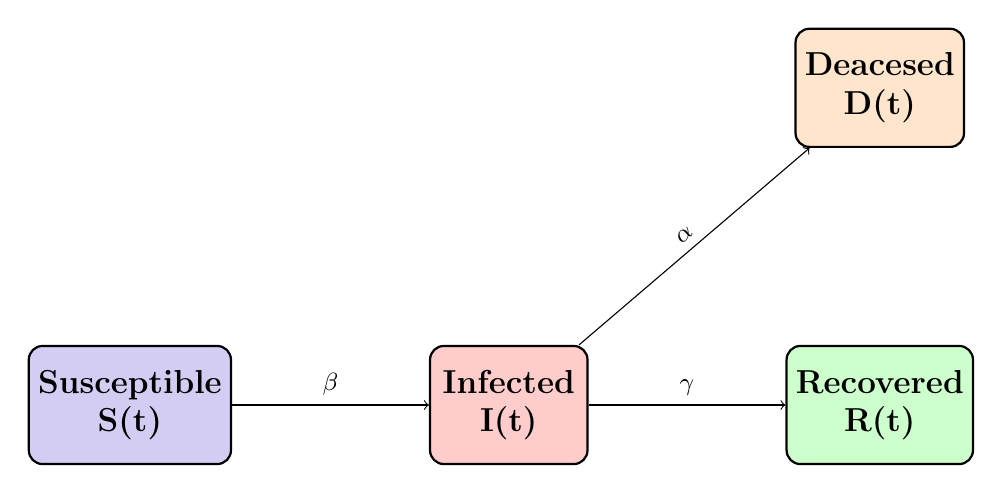
\begin{tikzpicture}[
    node distance=2.5cm,
    box/.style={rectangle, minimum width=2cm, minimum height=1.5cm, 
                draw=black, thick, align=center, rounded corners=5pt,
                font=\large\bfseries},
    arrow/.style={-Stealth, thick, line width=1.2pt},
    label/.style={midway, sloped, font=\small}
]

    % Define nodes
    \node[box, fill=blue!20] (S) {Susceptible \\ S(t)};
    \node[box, fill=red!20, right=of S] (I) {Infected \\ I(t)};
    \node[box, fill=green!20, right=of I] (R) {Recovered \\ R(t)};
    \node[box, fill=orange!20, right=of I, above=of R] (D) {Deacesed \\ D(t)};

    % Transitions
    \draw (S) edge[->] node[label,above] {$\beta$} (I);
    \draw (I) edge[->] node[label,above] {$\gamma$} (R);
    \draw (I) edge[->] node[label,above] {$\alpha$} (D);

\end{tikzpicture}
\caption{Grafo para o \textit{SIRD}. Fonte: elaborada pelos autores.}
\label{fig:sird-grafo}
\end{figure}

Outro exemplo é o \textit{SEIR} que inclui um compartimento para individuos que 
foram expostos a doença, mas ainda não manifestaram sintomas, ele é aplicável a 
doenças que possuem um tempo de latência entre o contanto com patogêneo e o surgimento
dos sintomas e capacidade do indivíduo de transmitir a doença. 

\begin{figure}[H]
\centering
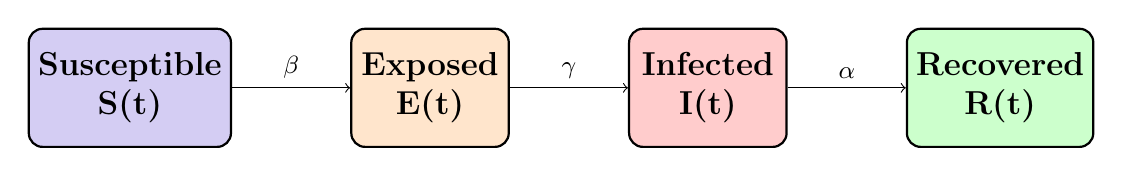
\begin{tikzpicture}[
    node distance=1.5cm,
    box/.style={rectangle, minimum width=2cm, minimum height=1.5cm, 
                draw=black, thick, align=center, rounded corners=5pt,
                font=\large\bfseries},
    arrow/.style={-Stealth, thick, line width=1.2pt},
    label/.style={midway, sloped, font=\small}
]

    % Define nodes
    \node[box, fill=blue!20] (S) {Susceptible \\ S(t)};
    \node[box, fill=orange!20, right=of S] (E) {Exposed \\ E(t)};
    \node[box, fill=red!20, right=of E] (I) {Infected \\ I(t)};
    \node[box, fill=green!20, right=of I] (R) {Recovered \\ R(t)};

    % Transitions
    \draw (S) edge[->] node[label,above] {$\beta$} (E);
    \draw (E) edge[->] node[label,above] {$\gamma$} (I);
    \draw (I) edge[->] node[label,above] {$\alpha$} (R);

\end{tikzpicture}
\caption{Grafo para o \textit{SEIR}. Fonte: elaborada pelos autores.}
\label{fig:seir-grafo}
\end{figure}

Compartimentos podem também ser removidos, como é o caso do modelo \textit{SIS}
apresentado no mesmo conjunto de trabalhos de Kermack e McKendrick 
\cite{kermack-mcKendrick-pt2:1932}, é um modelo com aplicação para doenças que 
não geram imunidade, como gripe e resfriado.  
Obviamente, é possível extender esse modelo, como é o caso do \textit{SEIS}, sendo
o \textit{SIS} com um compartimento para indivíduos expostos. 

\begin{figure}[H]
\centering
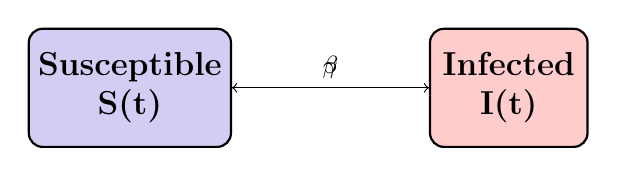
\begin{tikzpicture}[
    node distance=2.5cm,
    box/.style={rectangle, minimum width=2cm, minimum height=1.5cm, 
                draw=black, thick, align=center, rounded corners=5pt,
                font=\large\bfseries},
    arrow/.style={-Stealth, thick, line width=1.2pt},
    label/.style={midway, sloped, font=\small}
]

    % Define nodes
    \node[box, fill=blue!20] (S) {Susceptible \\ S(t)};
    \node[box, fill=red!20, right=of S] (I) {Infected \\ I(t)};

    % Transitions
    \draw (S) edge[->] node[label,above] {$\beta$} (I);
    \draw (I) edge[->] node[label,above] {$\gamma$} (S);

\end{tikzpicture}
\caption{Grafo para o \textit{SIS}. Fonte: elaborada pelos autores.}
\label{fig:sis-grafo}
\end{figure}

Compartimentos podem ser usados para modelar fenômenos específicos como a vacinação.
É o caso de modelos como o \textit{SIRV} \cite{schlickeiser-kroger:21-sirv} 
e o \textit{SIRVD}. Indivíduos são vacinados a uma taxa $\alpha$ e adquirem imunidade
à doença. Um parâmetro $\phi$ pode ser adicionado para dar conta de casos em que
a vacinação não é eficaz. 

\begin{figure}[H]
\centering
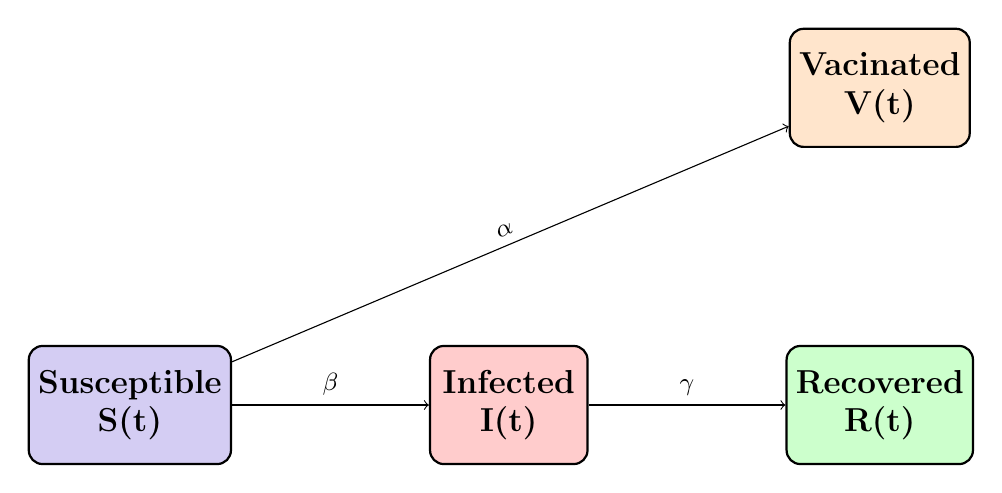
\begin{tikzpicture}[
    node distance=2.5cm,
    box/.style={rectangle, minimum width=2cm, minimum height=1.5cm, 
                draw=black, thick, align=center, rounded corners=5pt,
                font=\large\bfseries},
    arrow/.style={-Stealth, thick, line width=1.2pt},
    label/.style={midway, sloped, font=\small}
]

    % Define nodes
    \node[box, fill=blue!20] (S) {Susceptible \\ S(t)};
    \node[box, fill=red!20, right=of S] (I) {Infected \\ I(t)};
    \node[box, fill=green!20, right=of I] (R) {Recovered \\ R(t)};
    \node[box, fill=orange!20, right=of I, above=of R] (V) {Vacinated \\ V(t)};

    % Transitions
    \draw (S) edge[->] node[label,above] {$\beta$} (I);
    \draw (I) edge[->] node[label,above] {$\gamma$} (R);
    \draw (S) edge[->] node[label,above] {$\alpha$} (V);

\end{tikzpicture}
\caption{Grafo para o \textit{SIRV}. Fonte: elaborada pelos autores.}
\label{fig:sirv-grafo}
\end{figure}

Exemplos de modelos mais recentes, como o \textit{SVIHRD}, podem ser encontrados
em trabalhos como \cite{nelson-etal:24-japao}.
que inclui compartimentos para hospitalizados e vacinados e foi aplicado para 
modelar a pandemia de COVID-19. Outro exemplo é o \textit{SEIHDR}. 

\section{Variantes do Modelo SIR}

Ao longo dos anos foram propostas diferentes variantes do módelo \textit{SIR} original,
esta seção se dedica a abordar alguns exemplos brevemente. 
Em \cite{noble:1974-sir-difusao} é proposto uma variante do modelo que adiciona
uma variável espacial e cria um problema de difusão... 
Em \cite{singh-gupta:2022-generalized-sir} é proposto o Generalized SIR, GSIR...
Em \cite{andreu-vilarroig-etal:2025-sugestao-beta-t} é proposto um modelo que 
considera diferentes subcompartimentos para lidar com as diferentes ondas de 
influenza...
Outro exemplo que lida com as ondas de influenza \cite{lin:2003-sir-influenza}
Pode ser \cite{krylova:2013-sir-erlang}
    

\section{Aplicação de PINNs com Modelos Compartimentais}

Com a pandemia de COVID-19 no fim de 2019, renovou-se o interesse em modelos
epidemiológicos compartimentais. As PINNs, que haviam acabado de ser propostas,
foram encaradas como uma ferramenta nova que poderia ser utiizada junto com 
a grande quantidade de dados que estavam sendo gerados. 
Nesta seção são apresentados alguns trabalhos que aplicaram PINNs para solucionar
problemas em epidemiologia. São destacados novos modelos compartimentais, 
modificações feitas nos modelos clássicos, e aplicações inovadoras das PINNs.  

Em \cite{ouyoussef-etal:24-subcompartimentos} é apresentada uma variação
do \textit{SIR} em os compartimentos de suscetíveis e infectados 
são divididos em dois subgrupos. Há também um subgrupo de indivíduos 
vacinados \textit{V}, que assume constante ao longo do tempo do tempo, 
sendo que apenas uma porcentagem $\xi$ está totalmente imunizada.
Os autores não estavam interessados na taxa de recuperação, logo ela é assumida
como constante e a terceira equação do sistema \textit{SIR} é removida. 
A PINN passa a ter que aproximar as quatro curvas de interesse do modelo 
($S_1$, $S_2$, $I_1$, $I_2$), 
além de descobrir, as quatro taxas 
($\beta_{11}$, $\beta_{12}$, $\beta_{21}$ e $\beta_{22}$) de infecção
A aplicação destes subgrupos varia conforme a modelagem, 
pode se dividir a população por grupos de risco, por exemplo.
O modelo passaria a capturar as iterações entre estes subgrupos.
São feitos testes apenas com dados sintéticos. 

Outro exemplo utilizando subgrupos dentro dos compartimentos pode ser encontrado
em \cite{arulandu-etal:23-vacinacao}. Mas os autores vão além, ao utilizar 
o modelo de meta-populações de \cite{jacquez:1988-modelagam-hiv-matriz} que 
divide a população em $n$ subcompartimentos, transformando o parâmetro $\beta$ 
numa matriz $n \times n$. Através de simplificações algébricas, é proposto uma 
variação do \textit{SIR} com $3n$ equações e $3n + 3$ parâmetros.
Os autores então empregam este modelo junto com uma PINN para estimar o número 
de reprodução efetivo $R_i$ para cada população $i$, sendo $i \in [1,...,n]$. 
Este valor é então usado para ajudar na criação de um plano de vacinação que 
priorize populações mais vulneráveis, ou seja, aquelas em que $R_i$ é maior.
São realizados testes com a famosa base de dados sobre a dispersão de influenza
numa escola londrina.  

Modelos compartimentais utilizam sistemas de ODEs para modelar a evolução
de uma pandemia, considerando apenas o tempo como variável independente e 
ignorando a dimensão espacial.
Em \cite{bertaglia-etal:22-sir-reacao-difusao} é feita uma modificação do 
modelo \textit{SIR}, criando o \textit{SIR} hiperbólico. 
A modificação consiste em inser uma dimensão espacial e transformar o PVI
num problema de reação-difusão, numa EDP hiperbólica em função da dimensão espacial $x$
e temporal $t$. A função de perda da rede é modificada, mas tomando cuidado
para garantir que rede satisfaça a propriedades de convergência assintótica.
São realizados testes envolvendo problemas diretos e inversos para averiguar
a efetividade do modelo.

O uso de PINNs com modelos com mais compartimentos é explorado em \cite{nelson-etal:24-japao}.
O autores propõem o já mencionado \textit{SVIHRD}, um modelo que inclui 
compartimentos para vacinados (\textit{V}), hospitalizados (\textit{H}), 
e separa o compartimento de recuperados em entre os que se curaram e as 
fatalidades (\textit{D}).
O compartimento de hospitalizados é usado para medir a ocupação dos serviços de
saúde pública.
O modelo ainda inclui uma taxa de nascimentos para os 
suscetíveis e uma taxa de mortes naturais para todos os outros compartimentos.
É demonstrada a estabilidade do modelo e são feitos testes com dados da pandemia 
de COVID-19 no Japão.

Em \cite{han-etal:24-prim-artigo-alemanha} há um outro exemplo de aplicação de
PINNs com modelos comportimentais e parâmetros que variam no tempo. Os autores
aplicaram o modelo \textit{SAIRD} para gerar dados sintéticos para 
o treinamento de uma PINN. Uma vez validado o modelo, ele é utilizado para se
ajustar aos dados de COVID-19 da Alemanha. É feito um estudo sobre o
parâmetro $\omega_{\text{dados}}$ para diferentes valores e seus efeitos na 
convergência da rede e valores obtidos para os parâmetros do problema inverso. 

Um dos primeiros usos de PINNs com parâmetros variando no tempo é proposto em 
\cite{long-etal:21-L2}. Os autores aplicam uma PINN com o modelo \textit{SIRD}
para estimar a taxa de transmissão da COVID-19 em três cidades americanas
ao longo de março de 2020 a outrubro de 2020. Uma vez calculada a estimativa da 
taxa de transmissão ao longo do tempo, o número de reprodução básico é calculado
para o mesmo período. 
Os parâmetros estimados são alimentados numa \textit{Long Short Term Memory} 
(LSTM) para prever o número de infectados no mês seguinte, outubro. 

Em \cite{shamsara-etal:25-omicron} é apresentado uma aplicação de PINNs
junto ao modelo \textit{SVIHRD} com parâmetros variando no tempo. 
Os autores introduzem uma técnica para ajustar o peso $\omega_{\text{dados}}$ 
ao longo do treinamento da rede. O modelo é então aplicado
para ajustar a dados de COVID-19 dos países Itália, França e Alemanha. 
Uma vez estimada a taxa de transmissão da doença, ela é correlacionada com O
surgimento de variantes do vírus que causa a COVID-19.

Outra extensão feita nos modelos clássicos é proposta em \cite{nguyen-etal:22-raissi-seirp}.
Os autores modificam o \textit{SEIR} ao adicionar um compartimento $P$ para 
modelar a concentração de patogêneos em ambientes fechados, e a possibilidade
de contaminação pela doença através da interação não apenas com o contato com
individuos contaminados, mas também com a iteração com pantogêneos presentes no
ambiente. Os autores deduzem os pontos de equilíbrio do modelo e 
realizam testes com PINNs nos dados de influenza de um colègio
privado londrino.     

Um exemplo com modelos de ordem fracionária é apresentado em 
\cite{li-etal:25-ordem-fracionaria}. Os autores utilizam uma versão do 
\textit{SEIHDR} (\textit{Susceptible-Exposed-Invected-Hospitalized-Deacesed-Recovered}) 
com derivadas fracionárias de Caputo e parâmetros variando no tempo.
São feitas análises dos pontos de estabilidade do modelo, e o número de reprodução
básico é calculado utilizando matrizes de próxima geração. 
As PINNs são usadas para ajustar o modelo aos dados de COVID-19 do Canadá.

Em \cite{heldmann-etal:23-biobjective-opt} é aplicado o modelo \textit{SVIHRD}
com uma função de custo multi-objetivo ao tratar a $\mathcal{L}_{\text{física}}$
e a $\mathcal{L}_{\text{dados}}$ como duas funções objetivos distintas.
A função de perda da rede é composta por uma aproximação da curva Pareto entre 
as duas funções objetivos.
Outra inovação do artigo, é estimar alguns parâmetros utilizando o métedo de 
diferenças finitas alternativo. 
As PINNs são aplicadas para os dados de COVID-19 da Alemanha. São feitos ajustes
aos dados para estimar os parâmetros de transmissão e previsões de curto tempo.  

A combinação de modelos compartimentais com PINNs podem ser utilizados para 
outros fins que não apenas estimar a taxa de transmissão da doença.
Em \cite{ghosh-etal:23-subnotificacao} é apresentado uma variação do \textit{SEIR}
com níveis de imunidade dependentes do tempo e do número de doses de vacinas 
ministradas, o modelo também considera a eficácia da vacina. 
Estas adições ao \textit{SEIR} são modeladas na forma de parâmetros extras que 
podem mover indivíduos do compartimento de recuperados para o compartimento de
suscetíveis.
O modelo é aplicado junto a PINNs para estimar o nível de subnotificação de 
infectados e mortes não atribuídas a COVID-19 na China após o fim da política 
de COVID zero.

Outro exemplo que combina PINNs com métodos já consolidados na literatura
pode ser encontrado em \cite{millevoi-etal:24-split-join-pinns}.
Os autores propõem uma chamada "abordagem separada" (\textit{split approach}),
a ideia principal é separar o treinamento da rede em duas fases. Na primeira 
fase, o compartimento de infectados é aproximado utilizando uma rede neural
que se ajusta aos dados. Na segunda fase, a saída desta rede é então utilizada
junto a uma PINN para para estimar o número de suscetíveis e a taxa de transmissão
$\beta$ do modelo \textit{SIR}. A vantagem desta abordagem em comparação com a
abordagem tradicional, ou "conjunta" (\text{joint approach}) é simplificar a 
função de perda da rede neural ao simplificar as equações do modelo \textit{SIR}
que são usadas na função de perda, fazendo com que a PINN tenha uma curva a menos 
para se ajustar, melhorando a convergência da mesma. Os autores
testam a abordagem proposta com dados sintéticos e para dados de COVID-19 da Itália,
além de testes com lacunas nos dados para testar a resiliência da proposta. 

Em \cite{ogueda-oliva:23-colombia-duas-cidades} é feita uma modificação no
modelo \textit{SIRD} para modelar o descolocamento de pessoas duas 
cidades colombianas de Bogotá e Medellín. A incorporação deste movimento 
é feita através de uma matriz de transporte e o resultado é um modelo \textit{SIRD}
com duas populações distintas e, por consequência, dois compartimentos para cada
compartimento original ($S_1$, $S_2$, $I_1$, $I_2$, ...), assim como parâmetros 
duplicados ($\beta_1$, $\beta_2$, $\gamma_1$, $\gamma_2$, ...). O modelo é utilizado
para se ajustar aos dados de COVID-19 da Colômbia de 2021.

Em \cite{ning-etal:23-pinns-paralelas} são usadas PINNs paralelas para aproximar
cada compartimento do modelo \textit{SEIRD} com parâmetros variando no tempo.
Uma PINN pararela usa uma rede \textit{feedfoward} independente para aproximar 
cada saída da rede, ou para um conjunto de saídas. 
No artigo, os autores aproximam cada compartimento com uma rede independente, 
além de usar \textit{skip-connections} para previnir explosão e desaparecimento
de gradientes. 
As funções para os parâmetros $\beta$, $\gamma$ e $\mu$ são extraídos dos dos 
dados de COVID-19 da Itália em 2020 e são feitas previsões de curto prazo.
Os resultados obtidos com as PINNs são comparados com valores obtidos por métodos
Bayesianos. 

Outro exemplo de uso das PINNs paralelas é apresentado em  
\cite{yang-etal:25-dtpinns-paralelas}. Os autores propõem um modelo com 
comparimentos para vacinação e reinfecção, sendo que recuperados são movidos 
para uma compartimento $S_R$ e, caso infectados, movidos para um compartimento 
$I_2$. 
A itenção dos autores era demonstrar que a mortalidade entre reinfectados é maior 
do que entre os infectados.
Outra novidade, e a proposição das PINNs discretas, as \textit{dtPINNs}. A ideia
por de trás destas PINNs é utilizar uma rede neural para aproximar cada um dos 
parâmetro que variam no tempo, um método númerico, como o Runge-Kutta de quarta
ordem, é empregado para resolver o sistema de equações com os parãmetros que 
variam no tempo e com os parâmetros estáticos. 
A função de perda é calculada com base no \textit{MSE} entre a solução obtida pelo
método númerico e os dados. 
Os autores utilizam o método desenvolvido para estimar os parâmetros de COVID-19
do estado da Carolina do Norte, nos Estados Unidos.      

Em \cite{shaier-etal:22-dinns}, é feito um estudo dos efeitos de ruído nos dados
e dados faltantes na qualidade das soluções obtidas com PINNs para o modelo 
\textit{SIRD}.
Também  são realizados estudos dos efeitos de metaparâmetros como taxa de 
aprendizagem, número de pontos de colocação, largura das camadas escondidas e 
número de camadas escondidas.
PINNs são aplicadas juntas a vários modelos compartimentais para uma série de 
doenças como COVID-19, ebola, rubeola, pneumõnia, polio, dengue e zika. 

Em \cite{madden-etal:24-time-series-sir} é utilizada uma versão diferente do 
\textit{SIR} que utiliza séries temporais, o \textit{TSIR}.
A PINN utilizada tem uma entrada de alta dimensionalidade que incorpora dados
da população, retardos na transmissão da doença, dados sobre as cidades vizinhas.
O modelo desenvolvido é aplicado para os dados de sarampo da Inglaterra e do país
de Gales entre os anos de 1944 e 1965. Uma novidade deste artigo é tentar buscar
formas de inserir explicabilidade nas PINNs através de tecnicas como o
\textit{SHAP} (\textit{SHapley Additive exPlanations}).

Um exemplo de trabalho utilizando um modelo alternativo pode ser encontrado em
\cite{hu-etal:22-identificabilidade}, os autores aplicam o modelo \textit{SICDR} 
(\textit{Susceptible-Infected-Confirmed-Recovered-Deceased}).
Uma novidade apresentada nesse trabalho, é uma modificação na função de perda
da PINN que mantem a estabilidade do modelo, mesmo com compartimentos faltantes.
Outra abordagem inovadora é o uso de funções \textit{wavelet} para suavizar o 
ruído nos dados.
O modelo desenvolvido é aplicado para os dados de COVID-19 do Alabama no ano 
de 2020. 

Em \cite{schiassi-etal:21-xtfc} é proposto uma nova abordagem que combina PINNs
com uma técnica de interpolação chamada Teoria de Conexões Funcionais.
O algoritmo funciona aproximando funções por expressões condicionadas, uma expressão
condicionada uma é a soma de funções livres e um funcional que analiticamente satisfaz
as condições impostas não importando quais funções livres são escolhidas.
O modelo proposto é feito \textit{SIR}, \textit{SEIR} e \textit{SEIRS} 
(Susceptible-Exposed-Infectious-Recovered-Susceptible, um \textit{SEIR} com reinfecção). 
São feitos testes com dados sintéticos com e sem ruído.

Um exemplo utilizando redes neurais recorrentes pode ser encontrado 
em \cite{rodriguez-etal:2022-einns}. Os autores propõem uma \textit{framework} 
que combina uma rede \textit{feedfoward} informada pela física com redes recorrentes.
O intuito dos autores é desenvolver uma framework pensada para a previsão de 
tendências no desenvolvimento de uma pandemia a longo prazo incorporando dados 
das mais diversas fontes.

% No artigo original, são utilizados \textit{Multi-layer Perceptrons} (MLPs)
% como arquitetura das redes, mas há propostas com utilizando outras arquiteturas.
% Uma proposta utilizando redes neurais convolucionais pode ser encontrada em 
% \cite{shi-etal:24-convnet}. Uma proposta utilizando PINNs combinado com 
% métodos Bayesianos pode ser encontrada em \cite{yang:21-bpinns}, esta 
% abordagem é particulamente interessante para problemas inversos, ao transformar
% a estimativa dos parâmetros numa distribuição, no lugar de um valor fixo.

% % ==============================================================================
% TCC - Nome do Aluno
% Capítulo 2 - Revisão da Literatura
% ==============================================================================
\chapter{Revisão da Literatura}
\label{sec-literatura}

Neste capítulo é feita uma revisão dos principais conceitos utilizados neste
trabalho, além de apresentar fundamentos para uma compreensão mais profunda dos
mesmos.

\section{Redes Neurais Informadas pela Física}

Apresentadas em \cite{raissi-etal:19}, PINNs podem ser entendidas como uma forma
avançada de regularização, ou como um problema de otimização que transforma 
as condições de fronteira e iniciais em penalizações para a função custo. PINNs
são capazes de resolver problemas no seguinte formato: 

\begin{eqnarray}
    \mathcal{D}(u(\boldsymbol{x},t);\boldsymbol{\lambda}) &=& f(u,\boldsymbol{x},t), \quad \boldsymbol{x} \in \Omega, \, t \in I, \label{model-1-a}\\
    %
    \mathcal{B}(u(\boldsymbol{x},t)) &=& g(\boldsymbol{x},t), \quad \boldsymbol{x} \in \Gamma, \, t \in I, \label{model-1-b}\\
    %
    \mathcal{I}(u(\boldsymbol{x},t_0)) &=& q(\boldsymbol{x}), \quad \boldsymbol{x} \in \Omega, \label{model-1-c}
\end{eqnarray}

Em que $\Omega \subset \mathbb{R}^d$ é o domínio espacial limitado pela 
fronteira $\Gamma$; 
$d$ é a dimensão do domínio espacial; 
$T = [t_0, t_f]$ é o intervalo de tempo, sendo $t_0 < t_f$; 
$\boldsymbol{x} = (x_1, x_2, \dots, x_d)$ é um vetor de coordenadas espaciais; 
$t$ denota o tempo; 
$u = u(\boldsymbol{x}, t)$ denota a solução desconhecida do problema; 
$\boldsymbol{\lambda}$ é um vetor de parâmetros das equações; 
$\mathcal{D}$ é um operador diferencias associado às equações; 
$f$ é um termo fonte ou sorvedouro; 
$\mathcal{B}$ and $\mathcal{I}$ são operadores representando, respectivamente,
as condições de fronteira e iniciais; 
por fim, $g$ e $q$ são funções conhecidas que definem essas condições.

A equação \ref{eq:loss-fisica} define o termo da função de perda que engobla
todos as equações que compõem o modelo. Trata-se de um treinamento 
não-supervisionado que busca minimizar o residual definido.

\begin{equation}\label{eq:loss-fisica}
    \mathcal{L}_{\text{física}}(\boldsymbol{\theta}) 
    = \omega_{\text{domínio}} \mathcal{L}_{\mathcal{D}}(\boldsymbol{x},t,\boldsymbol{\theta}) 
    + \omega_{\text{fronteira}} \mathcal{L}_{\mathcal{B}}(\boldsymbol{x},t,\boldsymbol{\theta}) 
    + \omega_{\text{inicial}} \mathcal{L}_{\mathcal{I}}(\boldsymbol{x},t_0,\boldsymbol{\theta}) 
    %+ \omega_{data} J_{data}(\boldsymbol{x},t,\boldsymbol{\theta})
\end{equation}

Sendo $\omega_{\text{domínio}}$, $\omega_{\text{fronteira}}$ 
e $\omega_{\text{inicial}}$ pesos atribuídos a cada um dos residuais.
Caso haja dados disponíveis, é feito um treinamento supervisionado utilizando 
tais dados. A função de perda final da rede neural é então definida pela equação
\ref{eq:loss-total}.

\begin{eqnarray}\label{eq:loss-total} 
    \mathcal{L}_{\text{total}}(\boldsymbol{\theta}, \boldsymbol{\lambda}) 
    = \mathcal{L}_{\text{física}}(\boldsymbol{\theta}, \boldsymbol{\lambda}) 
    + \omega_{\text{dados}} \,\mathcal{L}_{\text{dados}}(\boldsymbol{\theta})
\end{eqnarray}

Aqui vale menciona que esta não é a única forma de distribuir os pesos da loss,
a implementação da biblioteca \textit{DeepXDE} \cite{lu-etal:21-deepxde}
permite atribuir pesos diferentes a cada condição inicial e de fronteira. 
Então o problema passa a ser encontrar os conjuntos $\boldsymbol{\theta}^*$ de 
parâmetros e viéses da rede, e o conjunto $\boldsymbol{\lambda}^*$ de parâmetros
das equações, que minimiza a função \ref{eq:loss-total}.

\begin{equation}\label{eq:otimizacao-parametros}
   (\boldsymbol{\theta}^*, \boldsymbol{\lambda}^*) 
   = \arg \min_{\boldsymbol{\theta}, \boldsymbol{\lambda}} \mathcal{L}_{\text{total}}(\boldsymbol{\theta}, \boldsymbol{\lambda}), 
\end{equation}

Existem muitos métodos de otimização para encontrar os argumentos 
da equação \ref{eq:otimizacao-parametros}. Pode-se citar o método de 
primeira ordem \textit{Adam} \cite{kingma-ba:14-adam} e o método quase-newtoniano
\textit{BFGS}, ou como comumente usado, a sua versão para ambientes de pouca
memória, o \textit{L-BFGS} \cite{liu-nocedal:89-lbfgs}.

A figura \ref{fig:pinn-representacao-grafica} mostra uma representação gráfica das 
PINNs.

\begin{figure}[htpb]
\centering
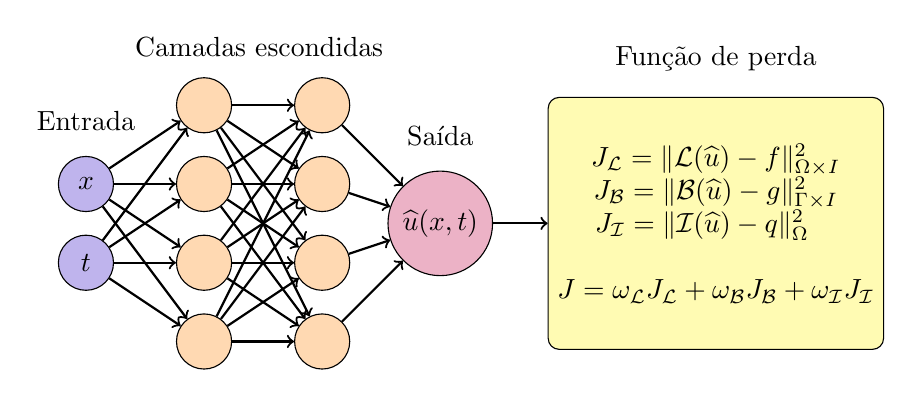
\begin{tikzpicture}[
    neuron/.style={circle, draw, minimum size=0.7cm},
    input/.style={neuron, fill=blue!30},
    hidden/.style={neuron, fill=orange!30},
    output/.style={neuron, fill=purple!30},
    physnode/.style={rectangle, draw, rounded corners, fill=orange!30, minimum width=1.5cm, minimum height=1.8cm},
    lossnode/.style={rectangle, draw, rounded corners, fill=yellow!30, minimum width=2cm, minimum height=3.2cm, align=center},
    every edge/.style={draw, ->, thick}
]

\node[input] (I-1) at (0, 2) {$x$};
\node[input] (I-2) at (0, 1) {$t$};

\node[hidden] (H1-1) at (1.5, 3) {};
\node[hidden] (H1-2) at (1.5, 2) {};
\node[hidden] (H1-3) at (1.5, 1) {};
\node[hidden] (H1-4) at (1.5, 0) {};

\node[hidden] (H2-1) at (3, 3) {};
\node[hidden] (H2-2) at (3, 2) {};
\node[hidden] (H2-3) at (3, 1) {};
\node[hidden] (H2-4) at (3, 0) {};

\node[output] (O-1) at (4.5, 1.5) {$\widehat{u}(x,t)$};

% Connections
\foreach \i in {1,2}
    \foreach \j in {1,...,4}
        \path (I-\i) edge (H1-\j);

\foreach \i in {1,...,4}
    \foreach \j in {1,...,4}
        \path (H1-\i) edge (H2-\j);

\foreach \j in {1,...,4}
    \path (H2-\j) edge (O-1);

\node[lossnode] (TotalLoss) at (8, 1.5) {
$J_{\mathcal{L}} = \lVert \mathcal{L}(\widehat{u}) - f \rVert^{2}_{\Omega \times I}$
\\
$J_{\mathcal{B}} = \lVert \mathcal{B}(\widehat{u}) - g \rVert^{2}_{\Gamma \times I}$
\\
$J_{\mathcal{I}} = \lVert \mathcal{I}(\widehat{u}) - q \rVert^{2}_{\Omega} \quad$
\\
\\
$J = \omega_{\mathcal{L}} J_{\mathcal{L}} + \omega_{\mathcal{B}} J_{\mathcal{B}} + \omega_{\mathcal{I}} J_{\mathcal{I}}$
};

\path (O-1) edge (TotalLoss);

% Labels
\node[above=0.2cm] at (I-1.north) {Entrada};
\node[above=0.2cm] at (2.2, 3.3) {Camadas escondidas};
\node[above=0.2cm] at (O-1.north) {Saída};
\node[above=0.2cm] at (TotalLoss.north) {Função de perda};

\end{tikzpicture}
\caption{Representação gráfica das PINNs. Fonte: elaborada pelos autores.}
\label{fig:pinn-representacao-grafica}
\end{figure}

A formulação acima vale tanto para problemas diretos, quanto para problemas 
inversos

\section{Modelos Compartimentais}

Baseados neste trabalho seminal,foram propostos outros modelos com mais mais 
compartimentos como o \textit{SEIRD} \cite{giles:77-sird} que inclui um 
compartimento para individuos que foram expostos a doença, mas 
ainda não manifestaram sintomas. 
Outro exemplo é o \textit{SIRV} \cite{schlickeiser-kroger:21-sirv} 
que inclui um compartimento para vacinados.

Em \cite{kendall:2023-modelos-epd-estocasticos}, é introduzido um modelo estocástico
baseado no trabalho já citado.

$R_0$ número básico

\begin{equation}
    R_0 = \frac{\beta}{\gamma}
\end{equation}

Apresentado no trabalho seminal de \cite{kermack-mcKendrick:1927}, o modelo 
\textit{SIR} é definido pelo conjunto de equações \ref{eq:SIR-1}, \ref{eq:SIR-2}
e \ref{eq:SIR-3}.

\begin{eqnarray}\label{eq:sir}
   \frac{dS(t)}{dt} &=& -\beta S(t) I(t),  \quad t > t_0, \label{eq:SIR-1}\\
   \frac{dI(t)}{dt} &=& \beta S(t) I(t) - \gamma I(t), \quad t > t_0, \label{eq:SIR-2}\\
   \frac{dR(t)}{dt} &=& \gamma I(t),  \quad t > t_0, \label{eq:SIR-3} \\
   S(t) + I(t) + R(t) &=& N,  \quad t > t_0, \label{eq:SIR-4}
\end{eqnarray}

O modelo pode ser entendido com um grafo\dots A figura \ref{fig:sir-grafo}
ilustra o modelo \textit{SIR}.

\begin{figure}
\centering
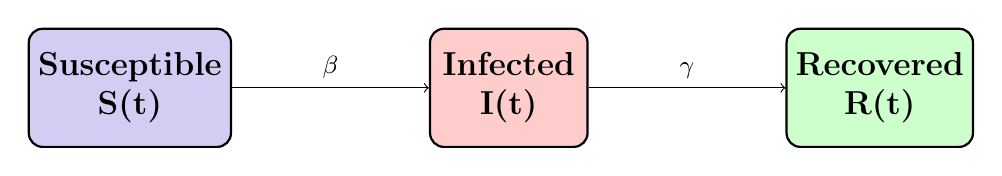
\begin{tikzpicture}[
    node distance=2.5cm,
    box/.style={rectangle, minimum width=2cm, minimum height=1.5cm, 
                draw=black, thick, align=center, rounded corners=5pt,
                font=\large\bfseries},
    arrow/.style={-Stealth, thick, line width=1.2pt},
    label/.style={midway, sloped, font=\small}
]

    % Define nodes
    \node[box, fill=blue!20] (S) {Susceptible \\ S(t)};
    \node[box, fill=red!20, right=of S] (I) {Infected \\ I(t)};
    \node[box, fill=green!20, right=of I] (R) {Recovered \\ R(t)};

    % Transitions
    \draw (S) edge[->] node[label,above] {$\beta$} (I);
    \draw (I) edge[->] node[label,above] {$\gamma$} (R);

\end{tikzpicture}
\caption{Grafo para o \textit{SIR}. Fonte: elaborada pelos autores.}
\label{fig:sir-grafo}
\end{figure}



\section{Problemas Inversos}

Problemas inversos são mal-postos\dots

Identificabilidade de um modelo\dots

\section{Aplicação de PINNs com Modelos Compartimentais}

\cite{}

Modelos de ordem facionária \cite{li-etal:25-ordem-fracionaria}

Sir reação-difusão \cite{bertaglia-etal:22-sir-reacao-difusao}

Um exemplo utilizando redes neurais recorrentes pode ser encontrado em \cite{rodriguez-etal:2022-einns}

No artigo original, são utilizados \textit{Multi-layer Perceptrons} (MLPs)
como arquitetura das redes, mas há propostas com utilizando outras arquiteturas.
Uma proposta utilizando redes neurais convolucionais pode ser encontrada em 
\cite{shi-etal:24-convnet}. Uma proposta utilizando PINNs combinado com 
métodos Bayesianos pode ser encontrada em \cite{yang:21-bpinns}, esta 
abordagem é particulamente interessante para problemas inversos, ao transformar
a estimativa dos parâmetros numa distribuição, no lugar de um valor fixo.

% ==============================================================================
% TCC - Nome do Aluno
% Capítulo 3 - Proposta do Trabalho
% ==============================================================================
\chapter{Proposta do Trabalho}
\label{sec-proposta}

Nesta seção é apresentada uma proposta para a estimativa dos parâmetros do 
modelo compartimental para dados epidemiológicos.
O modelo utilizado é apresentado, assim como a arquitetura da PINN utilizada.  
São também detalhados os testes para averiguar a efetividade do método.

\section{Estimativa de parâmetros}

Os modelos compartimentais possuem parâmetros de transmissão e mortalidade
fixos, considerando que estes modelos foram pensados apenas para dar 
uma projeção de como uma epidemia evoluirá. Entretanto, medidas de afastamento
social são capazes de alterar o parâmetro de transmissão ao longo do tempo.
Utilizando \cite{long-etal:21-L2} como inspiração, é proposto obter o parâmetro
$\beta$ como uma função em função do tempo. A rede neural deverá se ajustar 
a um $\beta(t)$. O modelo \textit{SIR} passa a ser escrito como, 

\begin{eqnarray}
   \frac{dS(t)}{dt} &=& -\frac{\beta(t) S(t)}{N} I(t),  \quad t > t_0, \label{eq:SIR-beta-t-1}\\
   \frac{dI(t)}{dt} &=& \frac{\beta(t) S(t)}{N} I(t) - \gamma I(t), \quad t > t_0, \label{eq:SIR-beta-t-2}\\
   \frac{dR(t)}{dt} &=& \gamma I(t),  \quad t > t_0, \label{eq:SIR-beta-t-3}
\end{eqnarray}

A taxa de mortalidade de um doença permanece a mesma para a maioria das doenças,
logo não há a necessidade de transformá-lo numa equação em função do tempo.
Considerando esse fato e seguindo o que foi aplicado em trabalhos como 
\cite{millevoi-etal:24-split-join-pinns} e \cite{ouyoussef-etal:24-subcompartimentos}, 
pode-se simplificar o sistama de equações acima, considerando que 
$S(t) + I(t) + R(t) = N$ para todo $t > t_0$.
A função $R(t)$ passa então a ser obtida pela subtração do total de individuos
na população pelos valores de $S(t)$ e $I(t)$.  

\begin{equation} \label{eq:Rt}
   R(t) = N - S(t) - I(t)
\end{equation}

A rede neural passar a ter que aproximar uma função $R \rightarrow R^3$ de 
$(S, I, \beta)$ em função de $t$ como ilustrado 
na figura \ref{fig:arquitetura-rede-solucao}.

\begin{figure}[htpb]
\centering
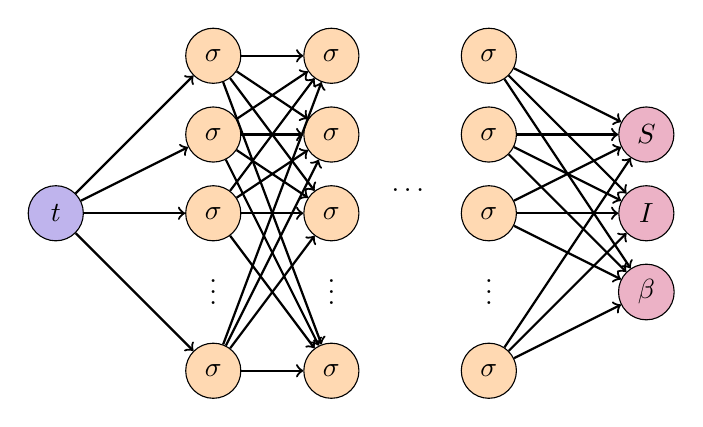
\begin{tikzpicture}[
    neuron/.style={circle, draw, minimum size=0.7cm},
    layer/.style={rectangle, minimum width=1.5cm, minimum height=8cm, draw=black, fill=blue!10, rounded corners=3pt},
    input/.style={neuron, fill=blue!30},
    hidden/.style={neuron, fill=orange!30},
    output/.style={neuron, fill=purple!30},
    physnode/.style={rectangle, draw, rounded corners, fill=orange!30, minimum width=1.5cm, minimum height=1.8cm},
    lossnode/.style={rectangle, draw, rounded corners, fill=yellow!30, minimum width=2cm, minimum height=3.2cm, align=center},
    every edge/.style={draw, ->, thick}
]

\node[input] (I-1) at (0, 2) {$t$};

\node[hidden] (H1-1) at (2, 4) {$\sigma$};
\node[hidden] (H1-2) at (2, 3) {$\sigma$};
\node[hidden] (H1-3) at (2, 2) {$\sigma$};
\node at (2, 1.1) {$\vdots$};
\node[hidden] (H1-4) at (2, 0) {$\sigma$};

\node[hidden] (H2-1) at (3.5, 4) {$\sigma$};
\node[hidden] (H2-2) at (3.5, 3) {$\sigma$};
\node[hidden] (H2-3) at (3.5, 2) {$\sigma$};
\node at (3.5, 1.1) {$\vdots$};
\node[hidden] (H2-4) at (3.5, 0) {$\sigma$};

\node at (4.5, 2.3) {$\dots$};

\node[hidden] (Hn-1) at (5.5, 4) {$\sigma$};
\node[hidden] (Hn-2) at (5.5, 3) {$\sigma$};
\node[hidden] (Hn-3) at (5.5, 2) {$\sigma$};
\node at (5.5, 1.1) {$\vdots$};
\node[hidden] (Hn-4) at (5.5, 0) {$\sigma$};

\node[output] (O-1) at (7.5, 3) {$S$};
\node[output] (O-2) at (7.5, 2) {$I$};
\node[output] (O-3) at (7.5, 1) {$\beta$};

% Connections

\foreach \j in {1,...,4}
    \path (I-1) edge (H1-\j);

\foreach \i in {1,...,4}
    \foreach \j in {1,...,4}
        \path (H1-\i) edge (H2-\j);

\foreach \i in {1,...,4}
    \foreach \j in {1,...,3}
        \path (Hn-\i) edge (O-\j);

\end{tikzpicture}
\caption{Representação gráfica das redes \textit{feedfoward}. Fonte: elaborada pelos autores.}
\label{fig:arquitetura-rede-solucao}
\end{figure}

\section{Justificativa para a Escolha do Modelo SIR}

O modelo \textit{SIR} pode não ser o melhor para os testes com dados reais de influenza,
entretanto, considerando o período de tempo em que o algoritmo foi executado não há 
necessidade de modelar a possibilidade de reinfecção. O motivo é que, apesar da gripe 
não gerar imunidade permanente, ainda assim gera imunidade por tempo suficiente
para poder ser desconsiderada pelo período de um ano. Logo não necessidade de usar
modelos como o \textit{SIRS} ou \textit{SIS}.  

\section{Testes com Dados Sintéticos}

Para averiguar se o método proposto funcionará bem com dados reais,
será feito primeiramente um teste com dados sintéticos obtidos a patir da solução
do modelo compartimental utilizando o método de Runge-Kutta de 4º ordem (RK4)
implementado na biblioteca \textit{SciPy} \cite{scipy}. O método resolverá 
o sistema de equações diferencias ao aproximar funções para os 3 compartimentos
do modelo \text{SIR} com o parãmetro $\beta$ em função do tempo. O único que 
será conhecido previamente, será justamente a função que descreve $\beta$.
Para emular um beta que varia em função do tempo, 
a função \ref{eq:beta_t_sintetetico} será utilizada.
\cite{andreu-vilarroig-etal:2025-sugestao-beta-t}
\cite{edlnd-etal:2011-sugestao-beta-t}.

\begin{equation} \label{eq:beta_t_sintetetico}
    \beta(t) = \sin(\frac{2\pi t}{t_f - t_0})  + \beta_{min}
\end{equation}

\begin{figure}[htpb]
\centering
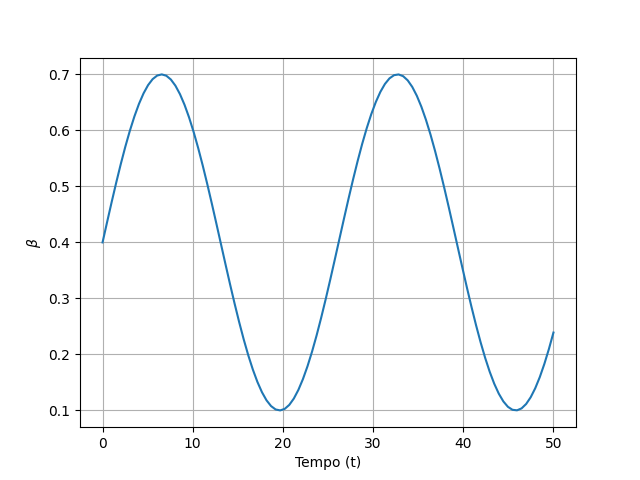
\includegraphics[width=0.6\textwidth]{figuras/real-beta-sir-nonoise.png}
\caption{Na primeira. Fonte: elaborada pelos autores.}
\label{fig:beta-sir-semruido}
\end{figure}

O modelo empregado é ligeiramente diferente do \textit{SIR} original. 
Será utilizada a sua forma normalizada, bastando remover o divisor $N$
das equações,

\begin{eqnarray}
   \frac{dS(t)}{dt} &=& -\beta(t) S(t) I(t),  \quad t > t_0, \label{eq:SIR-beta-t-1-norm}\\
   \frac{dI(t)}{dt} &=& \beta(t) S(t) I(t) - \gamma I(t), \quad t > t_0, \label{eq:SIR-beta-t-2-norm}\\
   \frac{dR(t)}{dt} &=& \gamma I(t),  \quad t > t_0, \label{eq:SIR-beta-t-3-norm}
\end{eqnarray}

Os compartimentos do modelo passam a ter um outro significado, não mostrado
mais o número de indivíduos em cada compartimento, mas sim a porcentagem 
da população que está em cada compartimento no instante $t$. 
Logo, a soma dos três compartimentos será igual a $1$ para todo instante $t$

\begin{equation}
    S(t) + I(t) + R(t) = 1, \quad t > t_0
\end{equation}

Levando isso em conta, as condições iniciais do problema são também expressadas
como porcentagens.

\begin{eqnarray}
   S_0 &=& 0.99 \label{eq:S0}\\
   I_0 &=& 0.01, \label{eq:I0}\\
   R_0 &=& 0 \label{eq:R0}
\end{eqnarray}

O problema é então resolvido para $t_0 \le t \ge t_f$, sendo $t_0=0$ e $t_f=50$.
A solução númerica obtida é então utilizada para obter um conjunto de 
$N_{data}$ valores para cada compartimento do modelo \textit{SIR}. 
Para este experimento, foram usados $100$ A figura \ref{fig:dados-semruido} 

\begin{figure}[htpb]
\centering
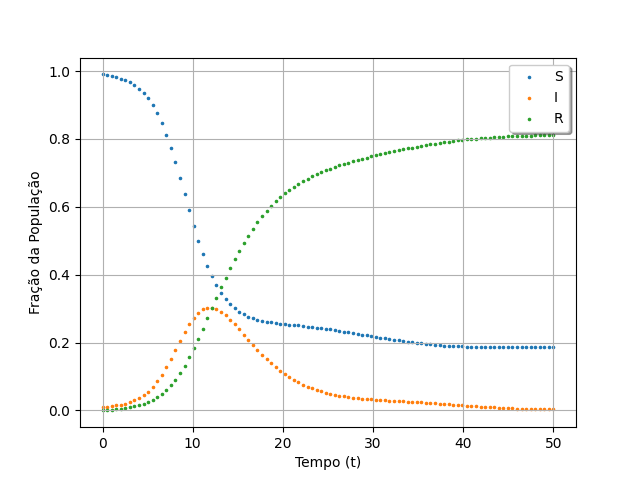
\includegraphics[width=0.6\textwidth]{figuras/runge-kutta-compartiments-data-sir-nonoise.png}
\caption{Na primeira. Fonte: elaborada pelos autores.}
\label{fig:dados-semruido}
\end{figure}

A solução com RK4 retorna dados para os três compartimentos, mas como a versão
do \textit{SIR} utilizada neste trabalho não possui a terceira equação, os 
dados para o terceiro compartimento (R) não são usados. Tomando como exemplo
trabalhos como \cite{han-etal:24-prim-artigo-alemanha} que utilizam apenas
dados do compartimento de infectados, mas conseguem bons resultados, o modelo
também será treinado apenas com dados sintéticos de incidência de infectados.  

\subsection{Avaliação dos Resultados}

A qualidade da solução obtida pela rede neural é medida pelo uso das métricas
de \textit{MSE}, norma euclidiana ($\mathcal{L}_2$) e norma no infinito 
($\mathcal{L}_{\infty}$). 
O \textit{MSE}, é definida pela equação \ref{eq:mse-metric}  

\begin{equation}\label{eq:mse-metric}
    \text{MSE} = \frac{1}{n} \sum_{i=1}^{n} (y_i - \hat{y}_i)^2
\end{equation}

A norma $\mathcal{L}_2$, é definida pela equação \ref{eq:l-2} e corresponde
a distância euclidiana entre as superfícies. È uma grandeza escalar  

\begin{equation}\label{eq:l-2}
    \mathcal{L}_2(\mathbf{x}, \mathbf{y}) = \|\mathbf{x} - \mathbf{y}\|_2 = \sqrt{\sum_{i=1}^{n} (x_i - y_i)^2}
\end{equation}

A norma $\mathcal{L}_{\infty}$, também chamada de norma máxima, é definida 
pela equação \ref{eq:l-infinity} e corresponde à distância máxima entre as
superfícies $\mathbf{x}$ e $\mathbf{y}$. A vantagem dessa métrica é mostrar
qual é o maior erro pontual. Uma desvantagem desta méstrica, é ser sensível 
a \textit{outliers}.

\begin{equation}\label{eq:l-infinity}
    \mathcal{L}_\infty(\mathbf{x}, \mathbf{y}) = \|\mathbf{x} - \mathbf{y}\|_\infty = \max_{i} |x_i - y_i|
\end{equation}

A comparação é feita com a solução númerica obtida com RK4 no caso dos 
compartimentos de sucetíveis e infectados. Para o parâmetro de taxa de infecção
$\beta$, a comparação é feita com a equação \ref{eq:beta_t_sintetetico}.

\section{Testes com Dados Sintéticos Ruidosos}

Segundo \cite{raissi-etal:19}, PINNs são resilientes a dados ruidosos. Para
testar se PINNs são capazes de corretamente aproximar as curvas do \textit{SIR}
mesmo com dados ruidosos,
é adicionado ruído gaussiano branco aos dados obtidos na seção anteior.
A equação \ref{eq:ruido-gaussiano} descreve este processo.

\begin{eqnarray}\label{eq:ruido-gaussiano}
    Z_t \sim \mathcal{N}(0, \sigma) \\
    \mathcal{N}_t = \max(\mathcal{C}_t + Z_t, 0)  
\end{eqnarray}

A figura \ref{fig:dados-comruido} mostra o resultado deste processo sobre os dados
de treinamento. Vale observar que para evitar usar dados negativos, pois são valores
que não fazem sentido no contexto do modelo, foi utilizada a função de máximo
entre o valor do dado de treinamento e zero.
Com este experimento, espera-se validar o método para a aplicação com dados reais,
que normalmente são pertubados. 

\begin{figure}[htpb]
\centering
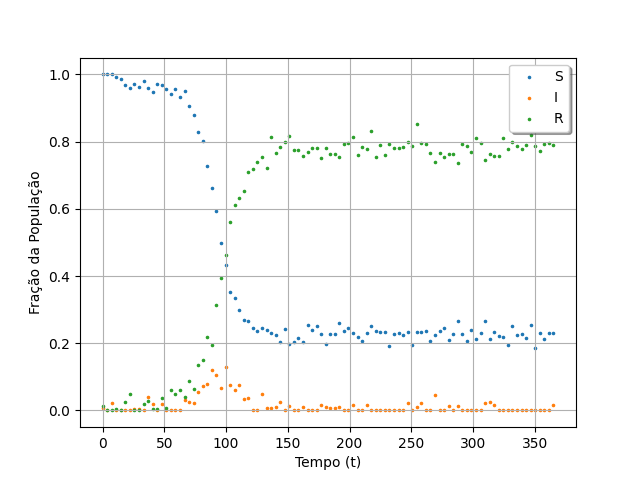
\includegraphics[width=0.6\textwidth]{figuras/runge-kutta-compartiments-data-sir-noisy.png}
\caption{Na primeira. Fonte: elaborada pelos autores.}
\label{fig:dados-comruido}
\end{figure}


\section{Testes com diferentes pontos de equilíbrio}

São feitos testes com diferentes pontos de equilíbrio livre de doença, pois uma 
vez atingindo este ponto de equilíbrio, a rede para de aproximar corretamente o 
valor de $\beta$. As figuras \ref{fig:dados-semruido-pe2} e \ref{fig:dados-comruido-pe2}
mostram os dados para o segundo ponto de equilíbrio para os casos de dados com
e sem ruído, respectivamente.  

\begin{figure}[htpb]
\centering
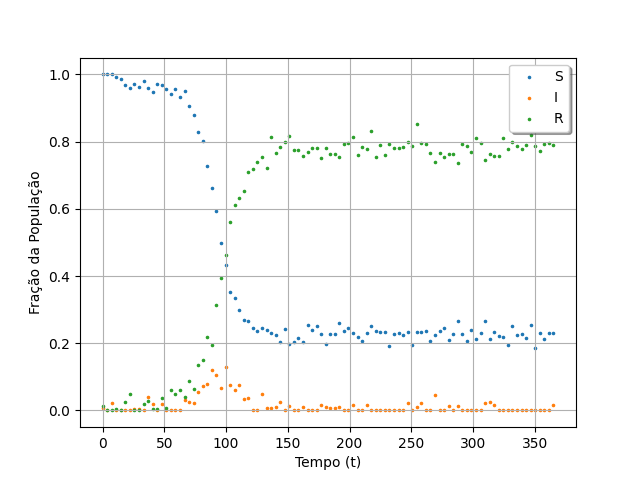
\includegraphics[width=0.6\textwidth]{figuras/runge-kutta-compartiments-data-sir-noisy.png}
\caption{Na primeira. Fonte: elaborada pelos autores.}
\label{fig:dados-semruido-pe2}
\end{figure}

\begin{figure}[htpb]
\centering
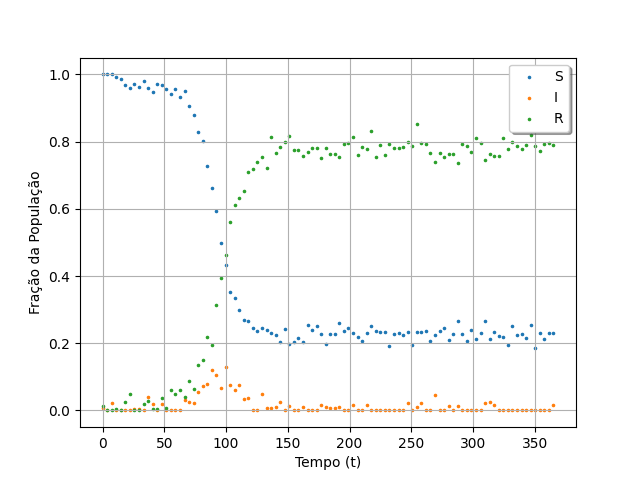
\includegraphics[width=0.6\textwidth]{figuras/runge-kutta-compartiments-data-sir-noisy.png}
\caption{Na primeira. Fonte: elaborada pelos autores.}
\label{fig:dados-comruido-pe2}
\end{figure}


\section{Testes com Base de Dados Reais}

São realizados testes utilizando dados reais...

\subsection{Base de dados da OMS}

Os dados foram coletados da plataforma \textit{FluNet} \cite{flunet}

\subsection{Bases de dados do DataSUS}

Os dados foram coletados do plataforma \textit{OpenDataSUS} \cite{opendatasus}

\subsection{Tratamento dos Dados}

\begin{figure}[htpb]
\centering
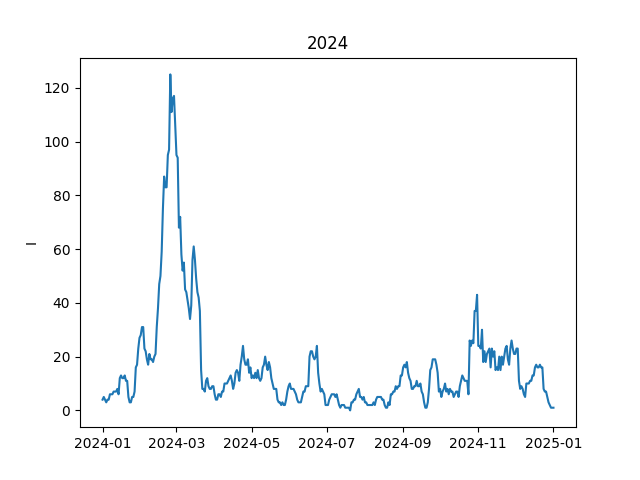
\includegraphics[width=0.6\textwidth]{figuras/data-2024-ES.png}
\caption{Na primeira. Fonte: elaborada pelos autores.}
\label{fig:dados-reais-sus-crus}
\end{figure}

Janela móvel de 7 dias como em \cite{han-etal:24-prim-artigo-alemanha},
\cite{long-etal:21-L2} e \cite{shamsara-etal:25-omicron} para suavizar o ruído


\begin{figure}[htpb]
\centering
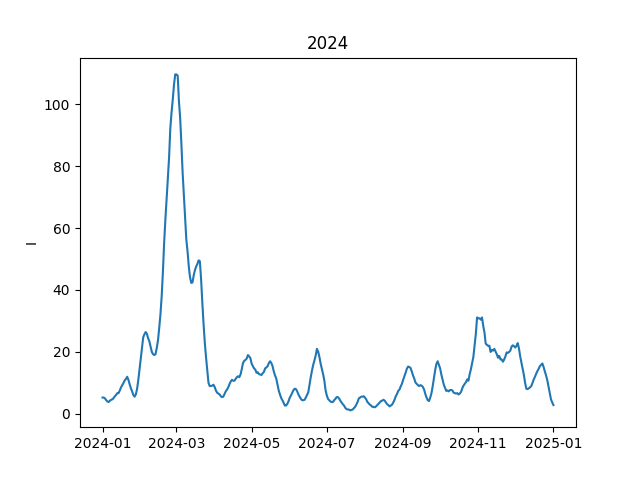
\includegraphics[width=0.6\textwidth]{figuras/smoothed-data-2024-ES.png}
\caption{Na primeira. Fonte: elaborada pelos autores.}
\label{fig:dados-reais-sus-media-movel}
\end{figure}

Pesos ajustáveis entre a loss física e a loss dos dados como em 
\cite{long-etal:21-L2} e 
\cite{shamsara-etal:25-omicron}

Segundo \cite{bonfanti-etal:24-generalizacao-pinns}, PINNs não generalizam bem
fora do domínio de treinamento. PINNs podem estimar os parâmetros para fora
do domínio de treinamento como em \cite{millevoi-etal:24-split-join-pinns}.

Assim como em \cite{ghosh-etal:23-subnotificacao}, fazer testes com lacunas
nos dados para testar a resiliência do método.

\section{Uso da Matriz de Nova Geração}

As condições inicial para os compartimentos \textit{Susceptible} e \textit{Infected}
podem ser facilmente determinadas pelo número total da populção e número de infectados
no primeiro dia. O mesmo não acontece para a taxa de transmissão $\beta$. Para 
estimar o valor $\beta_0$, foi utilizado método de matriz de nova geração.

\section{Arquitetura da Rede}

Baseando-se em \cite{shaier-etal:22-dinns}, o número de camadas escolhido foi...

Como em \cite{millevoi-etal:24-split-join-pinns}, aplicar uma 
\textit{hard-constraint} na rede neural ao utilizar nos nós de saída
uma função de ativação que retorna apenas valores positivos.

\subsection{Parâmetro  Ajustável}

Aplicando a ideia de \cite{shamsara-etal:25-omicron}, é adicionado uma parâmetros
$\omega_{\text{dados}}$ ajustável. 

\begin{equation}\label{eq:lambda-aprendivel}
    \omega_{\text{dados}} = \frac{max(\text{gradientes de }\mathcal{L}_{\text{física}})}{\text{média}(\text{gradientes de }\mathcal{L}_{\text{dados}})}
\end{equation}

\subsection{Regularização L2}

Seguindo os trabalhos de \cite{long-etal:21-L2} e \cite{shamsara-etal:25-omicron},
é aplicado uma regularização L2 na loss.

\begin{equation}\label{eq:regularizacao-L2}
    \mathcal{L}_2(\mathbf{x}, \mathbf{y}) = \|\mathbf{x} - \mathbf{y}\|_2 = \sqrt{\sum_{i=1}^{n} (x_i - y_i)^2}
\end{equation}

Os benefícios ligados ao uso da regularização L2 estão ligados a evitar gradientes
muito grandes, o que pode compromenter o processo de convergência da rede neural.

\subsection{Correlação com a Temperatura}

A gripe é uma doença com maior taxa de transmissão nos meses frios. 
Para testar se a transmissão em função do tempo aproximada pelo modelo é plausível,
é feito um teste de correlação de \textit{Pearson} entre $\beta(t)$ e a temperatura
ao longo do ano.

\subsubsection{Teste de Correlação de Pearson}

Sendo $\beta$ e $T$ duas amostras de tamanho $n$ com dados pareados $(\beta_i, T_i)$:
\begin{equation}\label{correlacao-de-pearson}
\rho = \frac{\sum_{i=1}^{n} (\beta_i - \bar{\beta})(T_i - \bar{T})}{\sqrt{\sum_{i=1}^{n} (\beta_i - \bar{\beta})^2 \sum_{i=1}^{n} (T_i - \bar{T})^2}}
\end{equation}

Espera-se um valor de $\rho$ acima de 0.5 para indicar um correlação no minímo moderada
entre a taxa de transmissão $\beta$ e a temperatura.

\subsubsection{Teste de Correlação de Spearman}

A correlação de Spearman é equivalent a calcular a correlação de Pearson nos 
\textit{ranks} dos valores.

\begin{equation}
r_s = \frac{\sum_{i=1}^{n} (R(\beta_i) - \bar{R_{\beta}})(R(T_i) - \bar{R_{T}})}{\sqrt{\sum_{i=1}^{n} (R(\beta_i) - \bar{R_{\beta}})^2 \sum_{i=1}^{n} (R(T_i) - \bar{R_T})^2}}
\end{equation}

Caso haja empates entre os elementos das amostras, aplica-se a fórmula de ajuste
abaixo.

\begin{equation}
r_s = \frac{\sum_{i=1}^{n} (R(\beta_i) - \bar{R_{\beta}})(R(T_i) - \bar{R_y})}{\sqrt{\left[\sum_{i=1}^{n} (R(x_i) - \bar{R_x})^2 - T_x\right]\left[\sum_{i=1}^{n} (R(y_i) - \bar{R_y})^2 - T_y\right]}}
\end{equation}

Sendo que os fatores $T_x$ e $T_y$ de correção de empate são calculados
usando as fórmulas abaixo.  

\begin{equation}
\mathcal{T} = \sum \frac{t^3 - t}{12}
\end{equation}


\section{Implementação e Execução}

A implementação foi feita utilizando a biblioteca \textit{DeepXDE} \cite{lu-etal:21-deepxde}, 
utilizando o \textit{TensorFlow} \cite{tensorflow:16} como \textit{backend}. 
Todo o código, dados utilizados nos experimentos,
encontram-se disponíveis no repositório público no 
GitHub\footnote{\url{https://github.com/ginbar/inverse-cm}}.
As sementes para a geração de pseudonúmeros foram fixadas para garantir
a reproducibilidade dos experimentos.

Todos os experimentos foram feitos numa máquina com 4GB de ram, processador
% ==============================================================================
% TCC - Nome do Aluno
% Capítulo 3 - Avaliação do Trabalho
% ==============================================================================
\chapter{Avaliação do Trabalho}
\label{sec-avaliacao}

\section{Testes com Dados Sintéticos}

A figura \ref{fig:compartimentos-sir-semruido} mostra o valor de 
beta ao longo do tempo.

\begin{figure}[htpb]
\centering
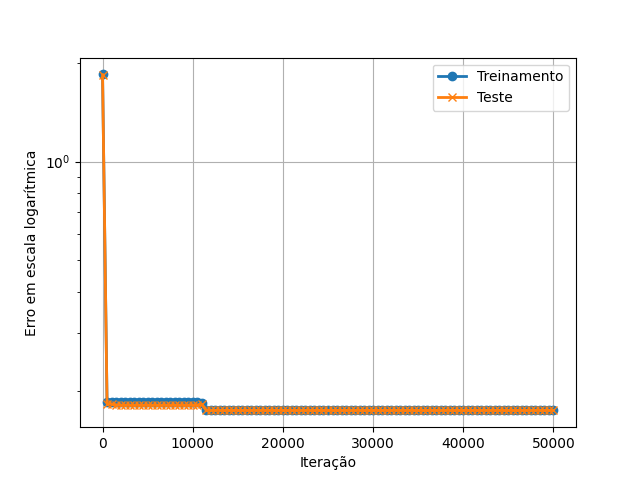
\includegraphics[width=0.6\textwidth]{figuras/loss-sir-nonoise.png}
\caption{Na primeira. Fonte: elaborada pelos autores.}
\label{fig:loss-sir-semruido}
\end{figure}


A figura \ref{fig:compartimentos-sir-semruido} mostra o valor de 
beta ao longo do tempo.

\begin{figure}[htpb]
\centering
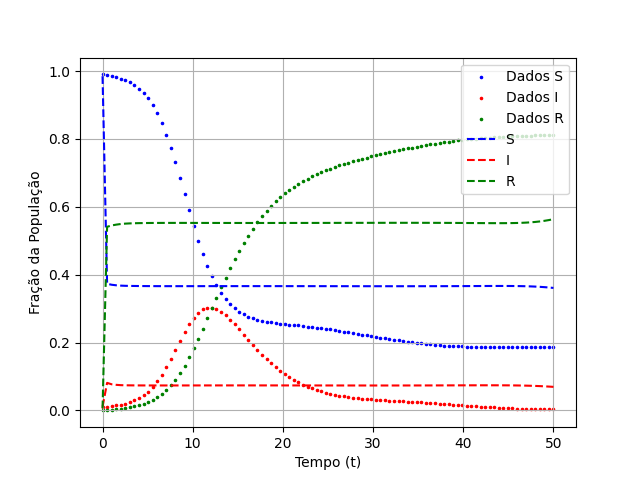
\includegraphics[width=0.6\textwidth]{figuras/predicted-compartments-sir-nonoise.png}
\caption{Na primeira. Fonte: elaborada pelos autores.}
\label{fig:compartimentos-sir-semruido}
\end{figure}

A figura \ref{fig:beta-sir-semruido} mostra o valor de beta ao longo do tempo.

\begin{figure}[htpb]
\centering
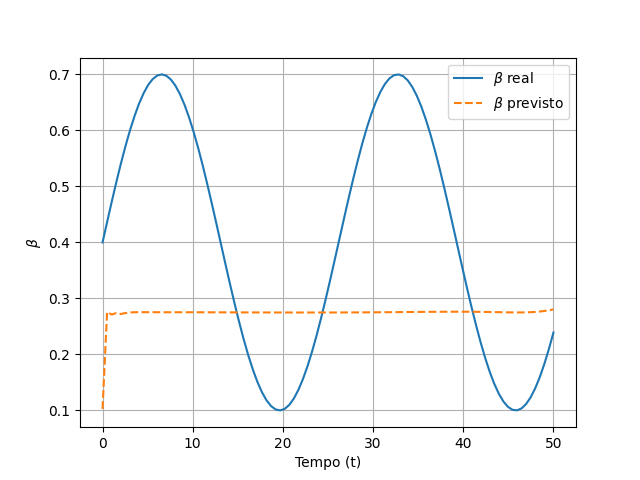
\includegraphics[width=0.6\textwidth]{figuras/predicted-beta-sir-nonoise.png}
\caption{Na primeira. Fonte: elaborada pelos autores.}
\label{fig:beta-sir-semruido}
\end{figure}


A tabela \ref{tab:metricas-dados-sinteticos} mostra os valores para 

\begin{table}[htpb]
\centering
\caption{Valores das métricas de erro (\textit{MSE}, norma $\mathcal{L}_2$ e norma $\mathcal{L}_\infty$) para as soluções aproximadas pela rede neural, em comparação com as soluções analíticas.}
\begin{tabular}{|c|c|c|c|}
\hline 
\hline 
\multirow{2}{*}{} & \multicolumn{3}{c|} {Métricas} \\ \cline{2-4} 
Compartimento & MSE & $\mathcal{L}_2$ & $\mathcal{L}_\infty$ \\ \hline
$S$ & $8{,}628 \times 10^{-6}$ & $2{,}444 \times 10^{-3}$ & $1{,}182 \times 10^{-2}$\\ \hline
$I$ & $1{,}005 \times 10^{-6}$ & $1{,}252 \times 10^{-2}$ & $4{,}81 \times 10^{-3}$\\ \hline
$R$ & $1{,}997 \times 10^{-6}$ & $4{,}913 \times 10^{-3}$ & $8{,}635 \times 10^{-3}$ \\ \hline
\hline
\end{tabular}
\label{tab:metricas-dados-sinteticos}
\end{table}


\section{Testes com Dados Ruidosos}

A figura \ref{fig:compartimentos-sir-semruido} mostra o valor de 
beta ao longo do tempo.

\begin{figure}[htpb]
\centering
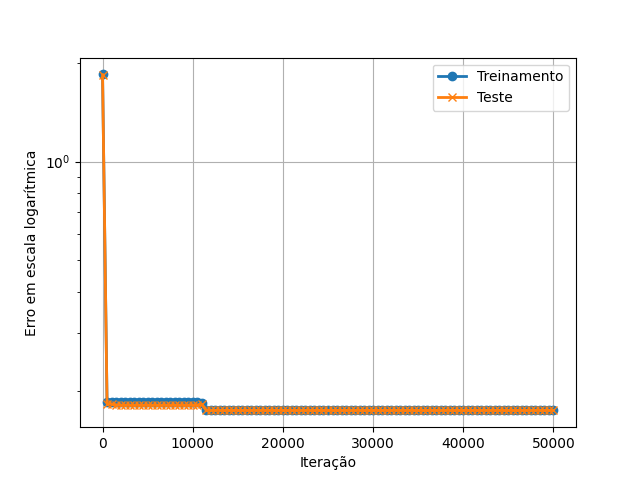
\includegraphics[width=0.6\textwidth]{figuras/loss-sir-nonoise.png}
\caption{Na primeira. Fonte: elaborada pelos autores.}
\label{fig:loss-sir-ruidoso}
\end{figure}


A figura \ref{fig:compartimentos-sir-ruidoso} mostra o valor de 
beta ao longo do tempo.

\begin{figure}[htpb]
\centering
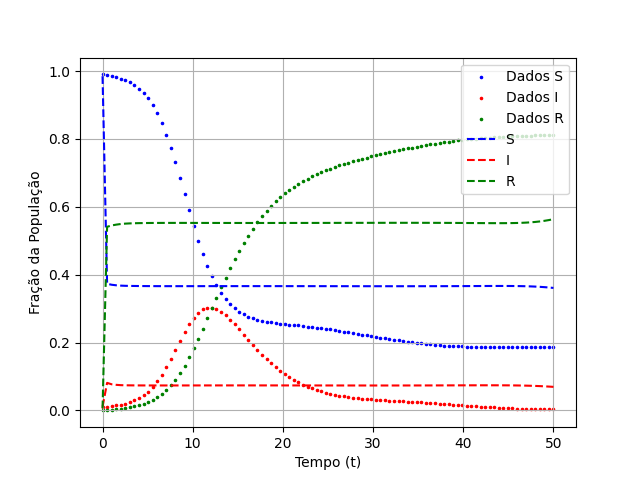
\includegraphics[width=0.6\textwidth]{figuras/predicted-compartments-sir-nonoise.png}
\caption{Na primeira. Fonte: elaborada pelos autores.}
\label{fig:compartimentos-sir-ruidoso}
\end{figure}

A figura \ref{fig:beta-sir-ruidoso} mostra o valor de beta ao longo do tempo.

\begin{figure}[htpb]
\centering
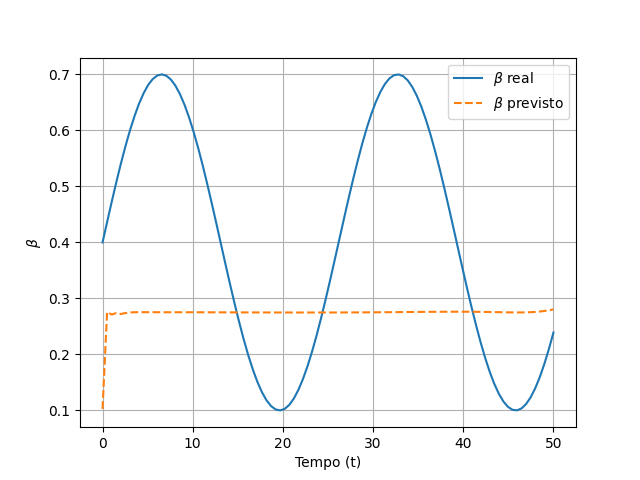
\includegraphics[width=0.6\textwidth]{figuras/predicted-beta-sir-nonoise.png}
\caption{Na primeira. Fonte: elaborada pelos autores.}
\label{fig:beta-sir-ruidoso}
\end{figure}


A tabela \ref{tab:metricas-dados-sinteticos-ruidosos} mostra os valores para 

\begin{table}[htpb]
\centering
\caption{Valores das métricas de erro (\textit{MSE}, norma $\mathcal{L}_2$ e norma $\mathcal{L}_\infty$) para as soluções aproximadas pela rede neural, em comparação com as soluções analíticas.}
\begin{tabular}{|c|c|c|c|}
\hline 
\hline 
\multirow{2}{*}{} & \multicolumn{3}{c|} {Métricas} \\ \cline{2-4} 
Compartimento & MSE & $\mathcal{L}_2$ & $\mathcal{L}_\infty$ \\ \hline
$S$ & $8{,}628 \times 10^{-6}$ & $2{,}444 \times 10^{-3}$ & $1{,}182 \times 10^{-2}$\\ \hline
$I$ & $1{,}005 \times 10^{-6}$ & $1{,}252 \times 10^{-2}$ & $4{,}81 \times 10^{-3}$\\ \hline
$R$ & $1{,}997 \times 10^{-6}$ & $4{,}913 \times 10^{-3}$ & $8{,}635 \times 10^{-3}$ \\ \hline
\hline
\end{tabular}
\label{tab:metricas-dados-sinteticos-ruidosos}
\end{table}

\section{Testes com Base de Dados Reais}
% ==============================================================================
% TCC - Nome do Aluno
% Capítulo 3 - Considerações Finais
% ==============================================================================
\chapter{Considerações Finais}
\label{sec-conclusoes}

Aplicar PINNs Bayesianas \cite{yang:21-bpinns} para estimar o desvio 
padrão do $\beta(t)$.




%%% Páginas finais do documento: bibliografia e anexos. %%%

% Finaliza a parte no bookmark do PDF para que se inicie o bookmark na raiz e adiciona espaço de parte no sumário.
\phantompart

% Marca o início dos elementos pós-textuais.
\postextual

% Referências bibliográficas
\bibliography{bibliografia}


% Apêndices.
\begin{apendicesenv}

% Imprime uma página indicando o início dos apêndices.
\partapendices

% (*) Incluir como apêndice a documentação técnica produzida durante o TCC (especificação de requisitos,
% projeto arquitetural, etc.). Utilizar o exemplo \includepdf caso o documento seja produzido em outro
% editor de texto (Microsoft Word, LibreOffice Writer) e transformado em PDF. Utilizar o exemplo \include
% caso os documentos tenham sido também escritos em LaTeX.
% \includepdf[pages={1-}]{apendices/apendice01-requisitos.pdf}
% \includepdf[pages={1-}]{apendices/apendice02-projeto.pdf}
% \include{ap1-requisitos}
% \include{ap2-projeto}
\end{apendicesenv}


% Índice remissivo.
\phantompart
\printindex

% Fim do documento.
\end{document}
